\defChapterTarget{Design-in-the-small}
    \section{Commenti}
    In questa sezione presentiamo il design in-the-small di elementi principali
    del sito. Ogni pagina contiene un header e un footer. L'header contiene
    sempre i link a elmenti fondamentali del sito web: I nostri servizi, Chi
    siamo, Le nostre news, I nostri volontari, I nostri eventi, Sostienici.
    L'header contiene sempre: Contattaci, Raggiungici e Lavora con noi.
    \section{I nostri volontari}
    La pagina "I nostri volontari" è una delle principali pagine del sito e
    mostra tutti i volontari dell'associazione. I volontari sono caricati dal
    database e mostrati grazie a una fotografia con il nome. Nella parte destra
    della pagina è presente una barra di ricerca che permette di ricercare il
    volontario scrivendo il nome. Sotto la barra di ricerca sono presenti dei
    filtri che permettono di mostrare solo dei volontari che hanno un profilo
    comune come "Studenti" o "Professori". Cliccando sulla fotografia del
    volontario è possibile raggiungere la pagina del singolo volontario
    sfruttando un apposito group link.

        \subsection{I nostri volontari in-the-small}
        \begin{figure}[H]
            \centering
            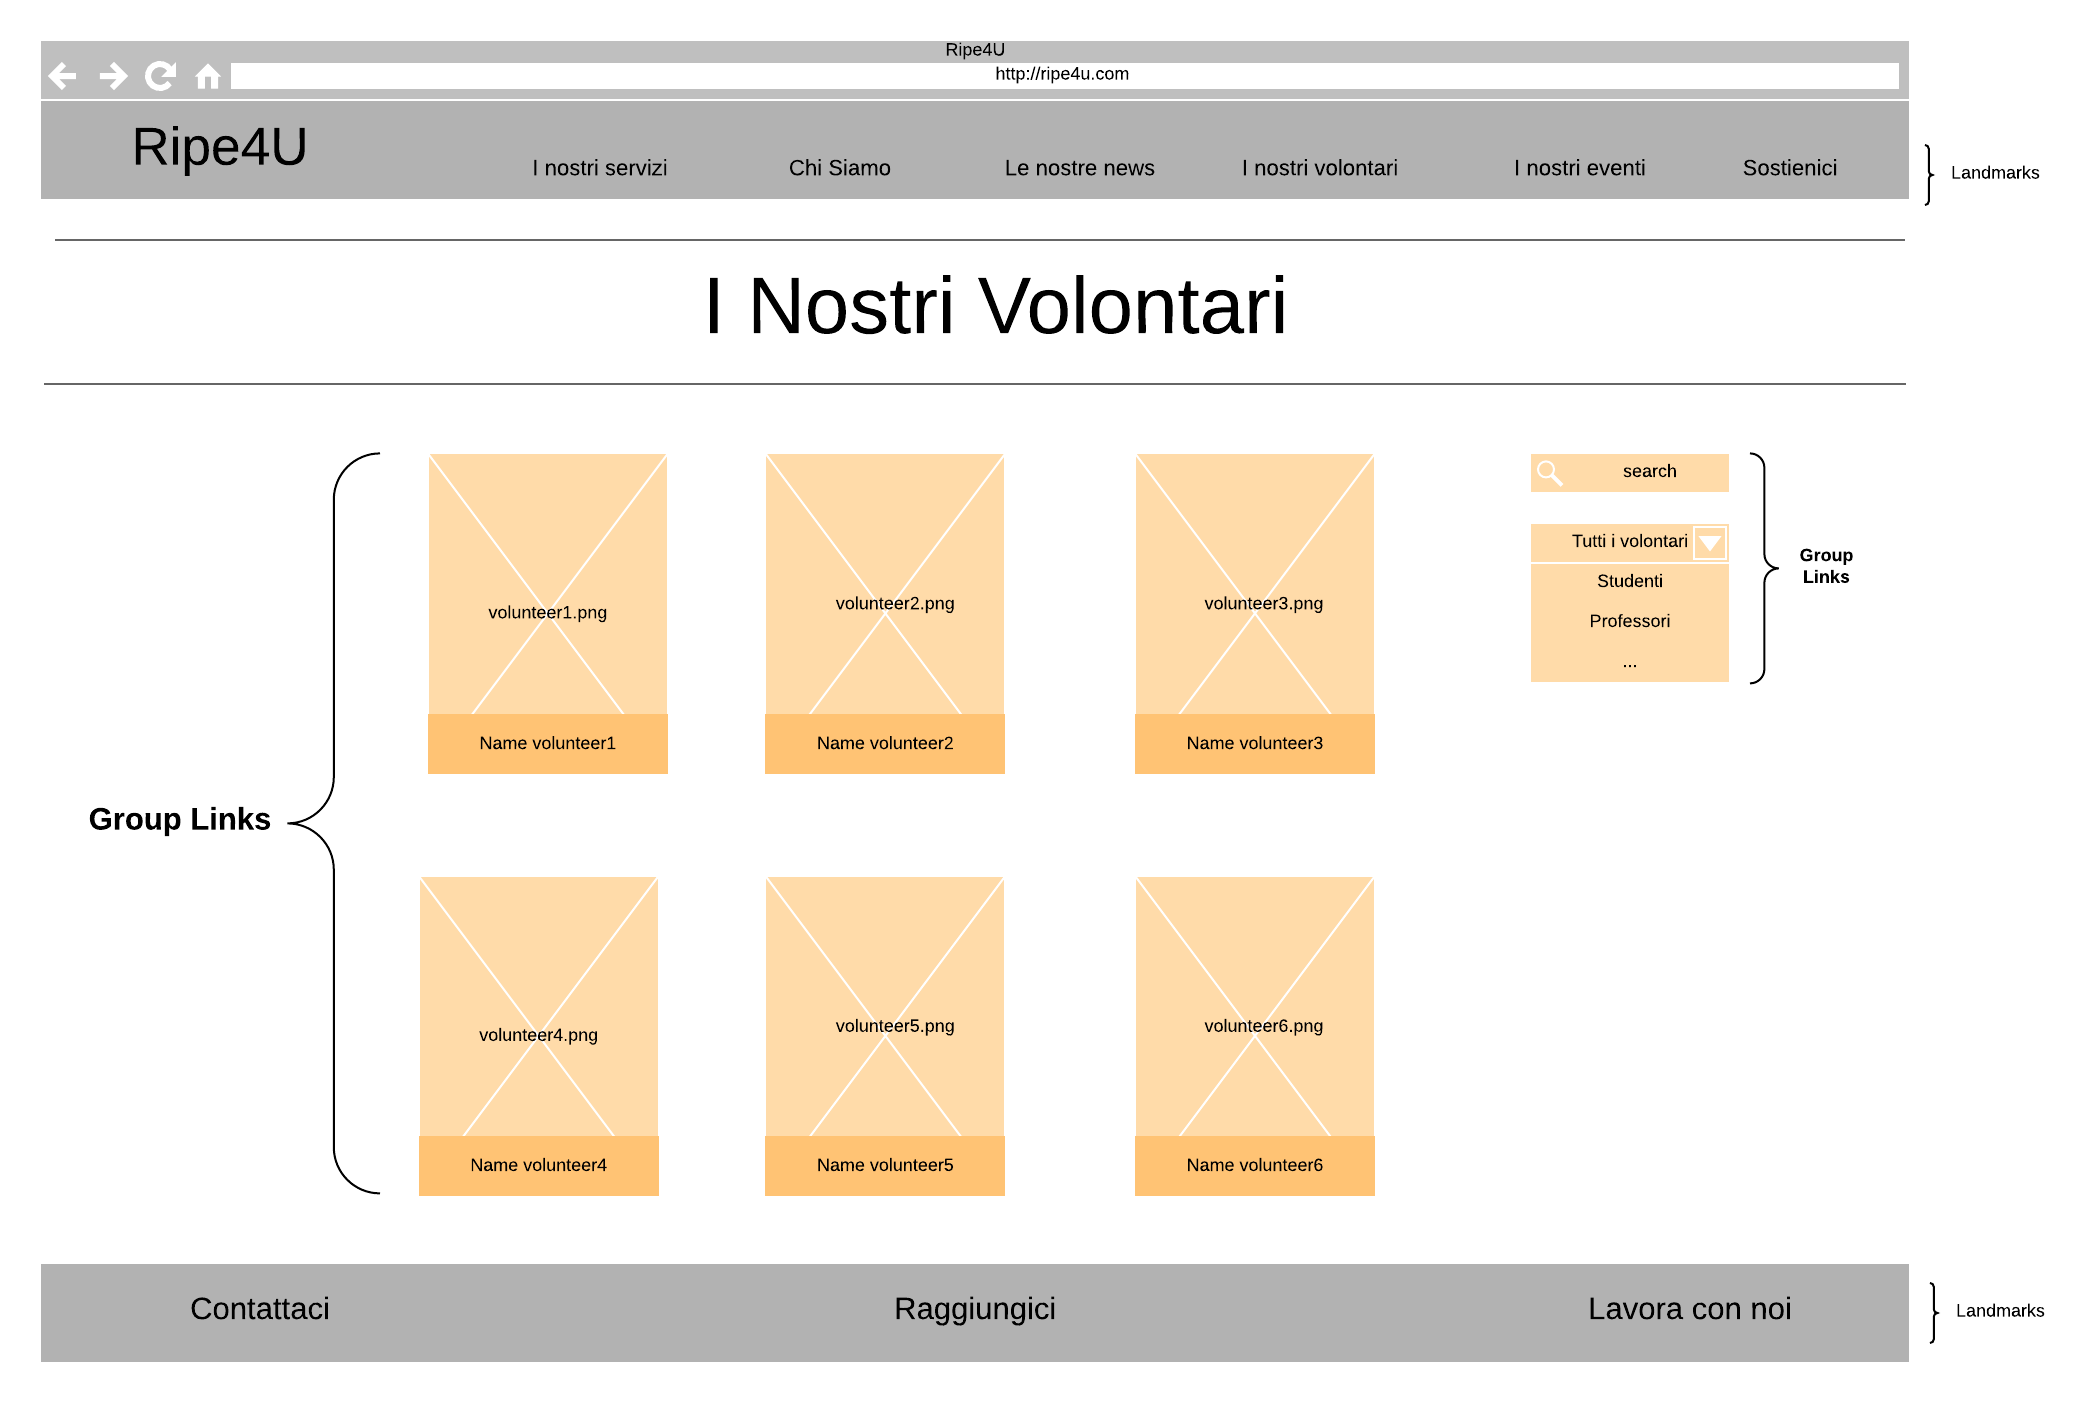
\includegraphics[scale=0.40]{resources/images/iNostriVolontari-in-the-small.jpg}
        \end{figure}

        \subsection{I nostri volontari mockup}

    \section{Volontario}
    Questa pagina permette di avere informazioni riguardo al singolo volontario.
    Come primo elemento vediamo la sua fotografie e immediatamente sotto due
    colonne. A destra e a sinistra della foto sono presenti due group link che
    permettono di vedere il volontario precedente e successivo. Nella colonna di
    sinistra sotto la foto c'è una descrizione del volontario seguita dalla sua
    carriera ed esperienze. In basso ci sono i contatti come ad esempio il
    numero di telefono o la e-mail per raggiungere il volontario. Nella colonna
    di sinistra sono presente i servizi e gli eventi in cui è coinvolto che
    possono essere cliccati sfruttando dei Transition links per avere ulteriori
    informazioni.

        \subsection{Volontario in-the-small}
        \begin{figure}[H]
            \centering
            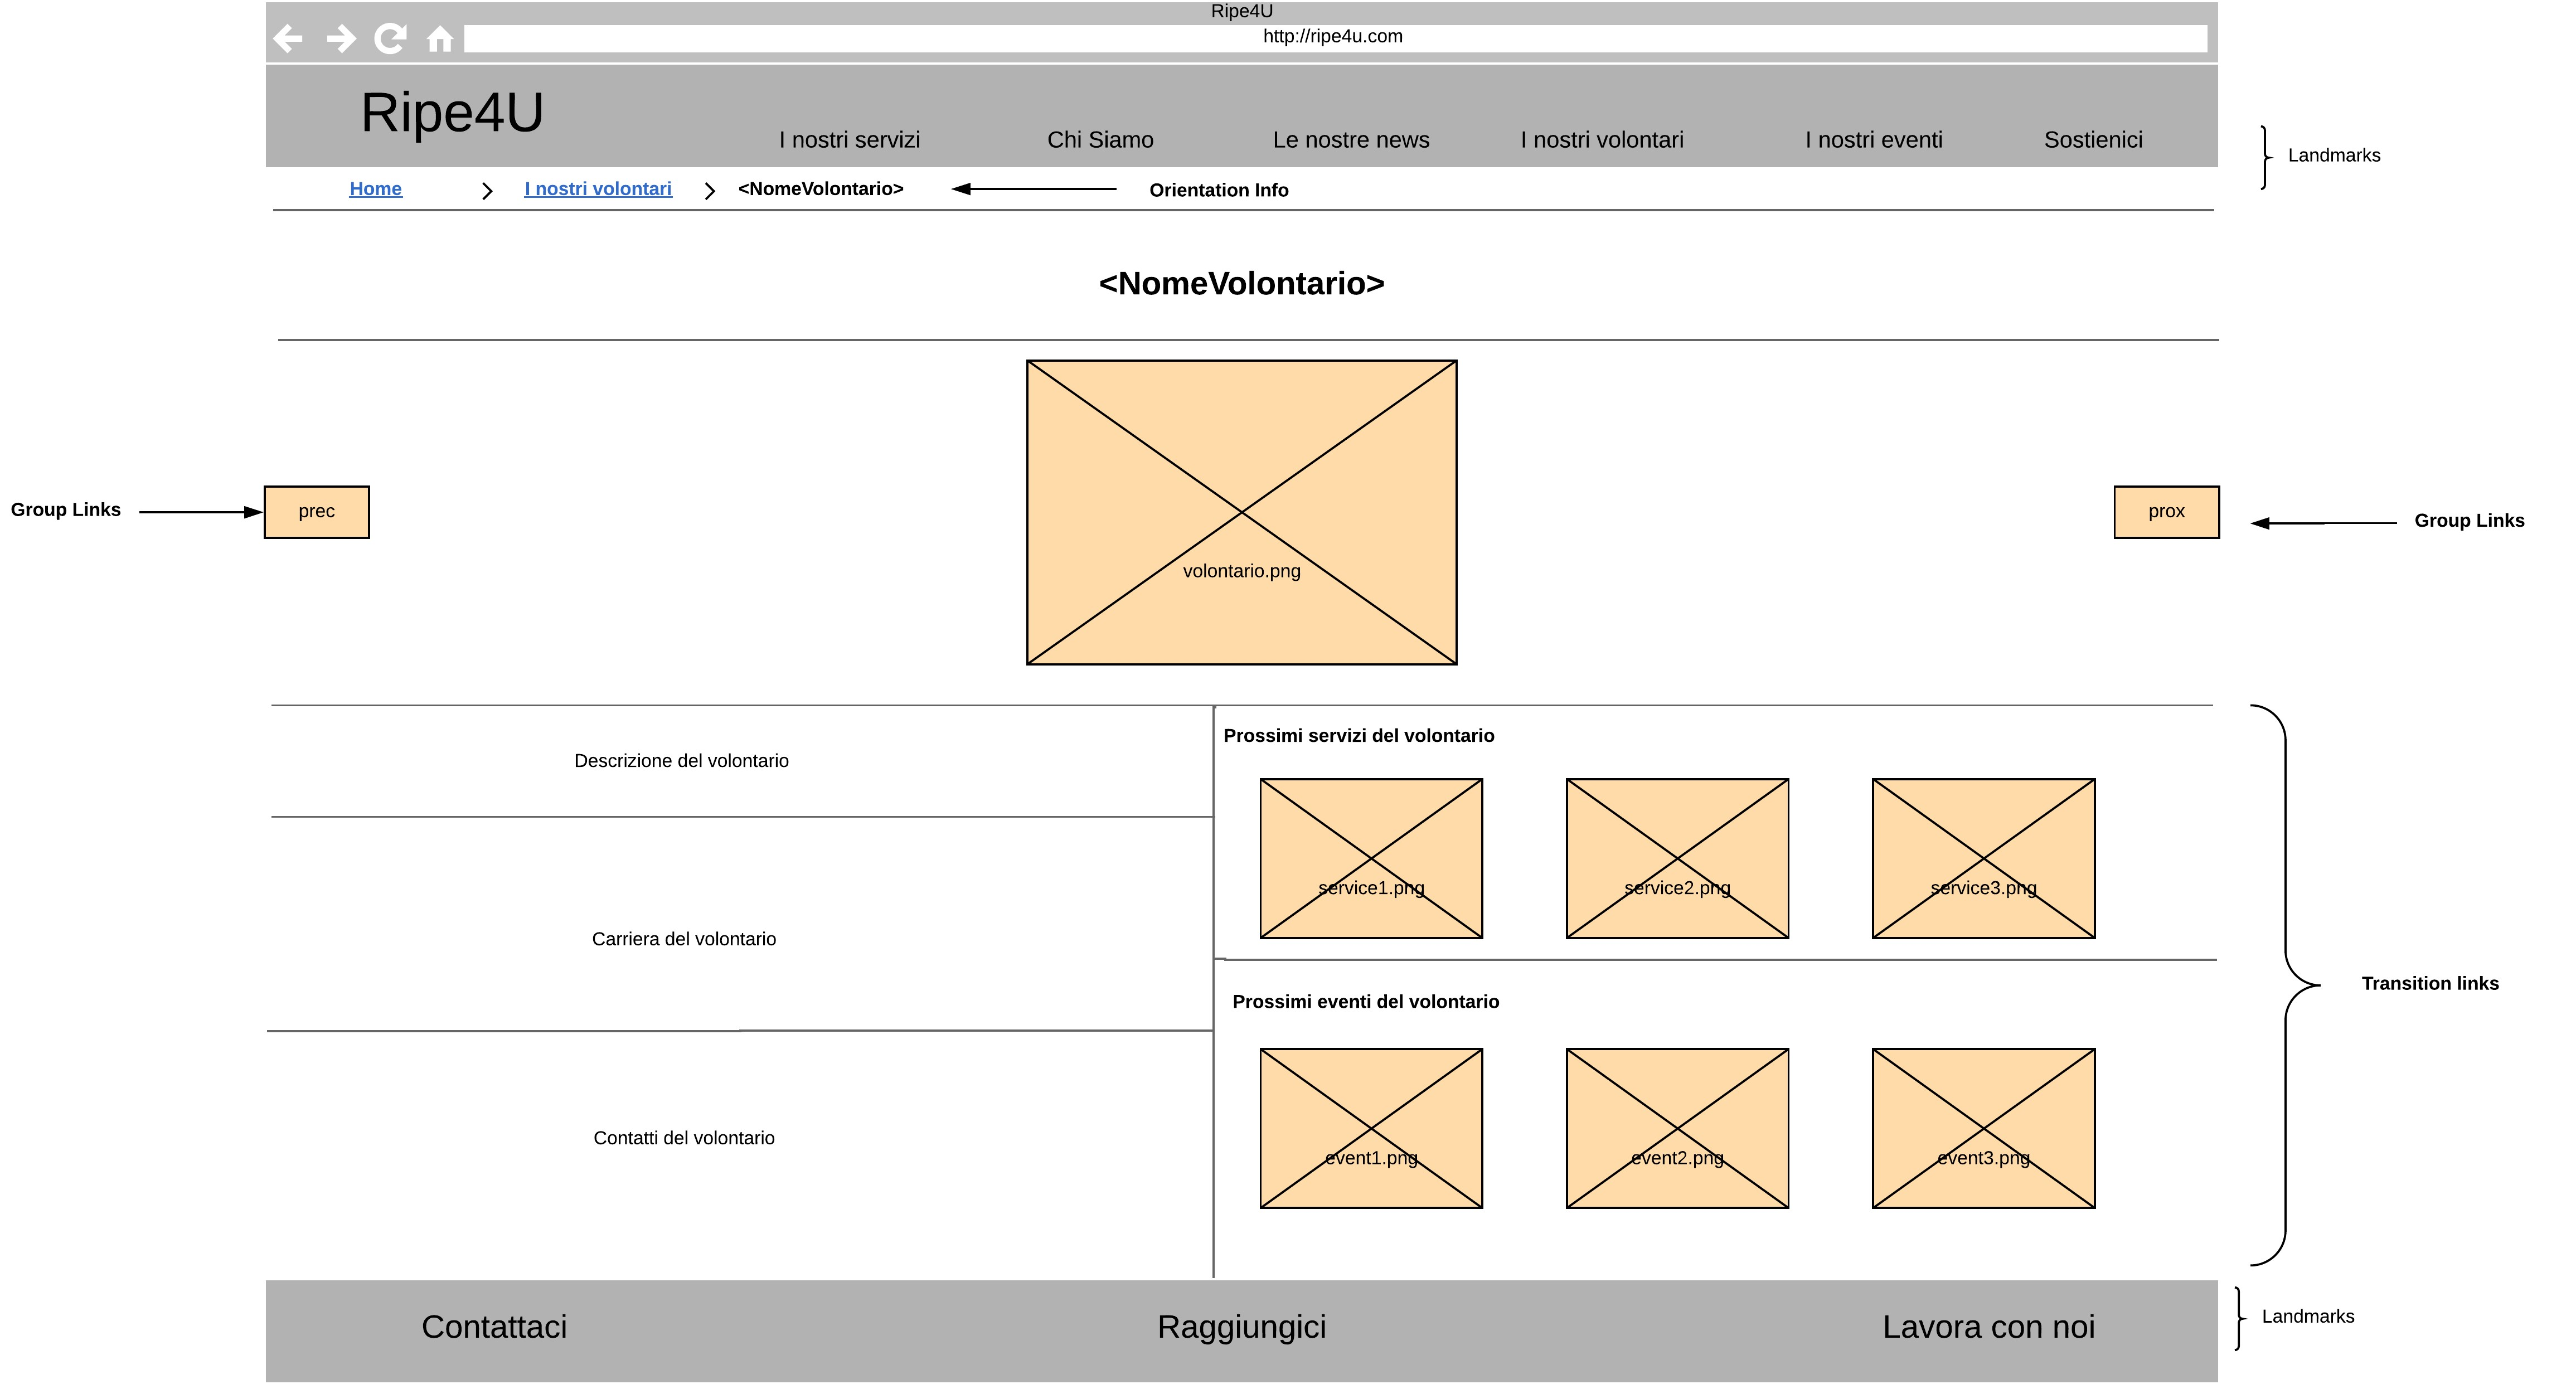
\includegraphics[scale=0.38]{resources/images/volontario-in-the-small.jpg}
        \end{figure}

        \subsection{Volontario mockup}

    \section{I nostri servizi}
    La pagina "I nostri servizi" è sicuramente la pagina principale del sito e
    mostra tutti i servizi che i volontari offrono alle persone. Sono presenti
    delle foto esplicative con il nome del servizio. Nella parte destra della
    pagina è presente una barra di ricerca che permette di cercare un servizio
    specifico come ad esempio "ripetizioni matematica". Sotto la barra di
    ricerca sono presenti dei filtri che permettono di mostrare i servizi in
    base alla tipologia come ad esempio "Ripetizioni" o "Orientamento".
    Cliccando sulle fotografie è possibile raggiungere la pagina del singolo
    servizio, sfruttando un apposito group link.
        \subsection{I nostri servizi in-the-small} 
        \begin{figure}[H]
            \centering
            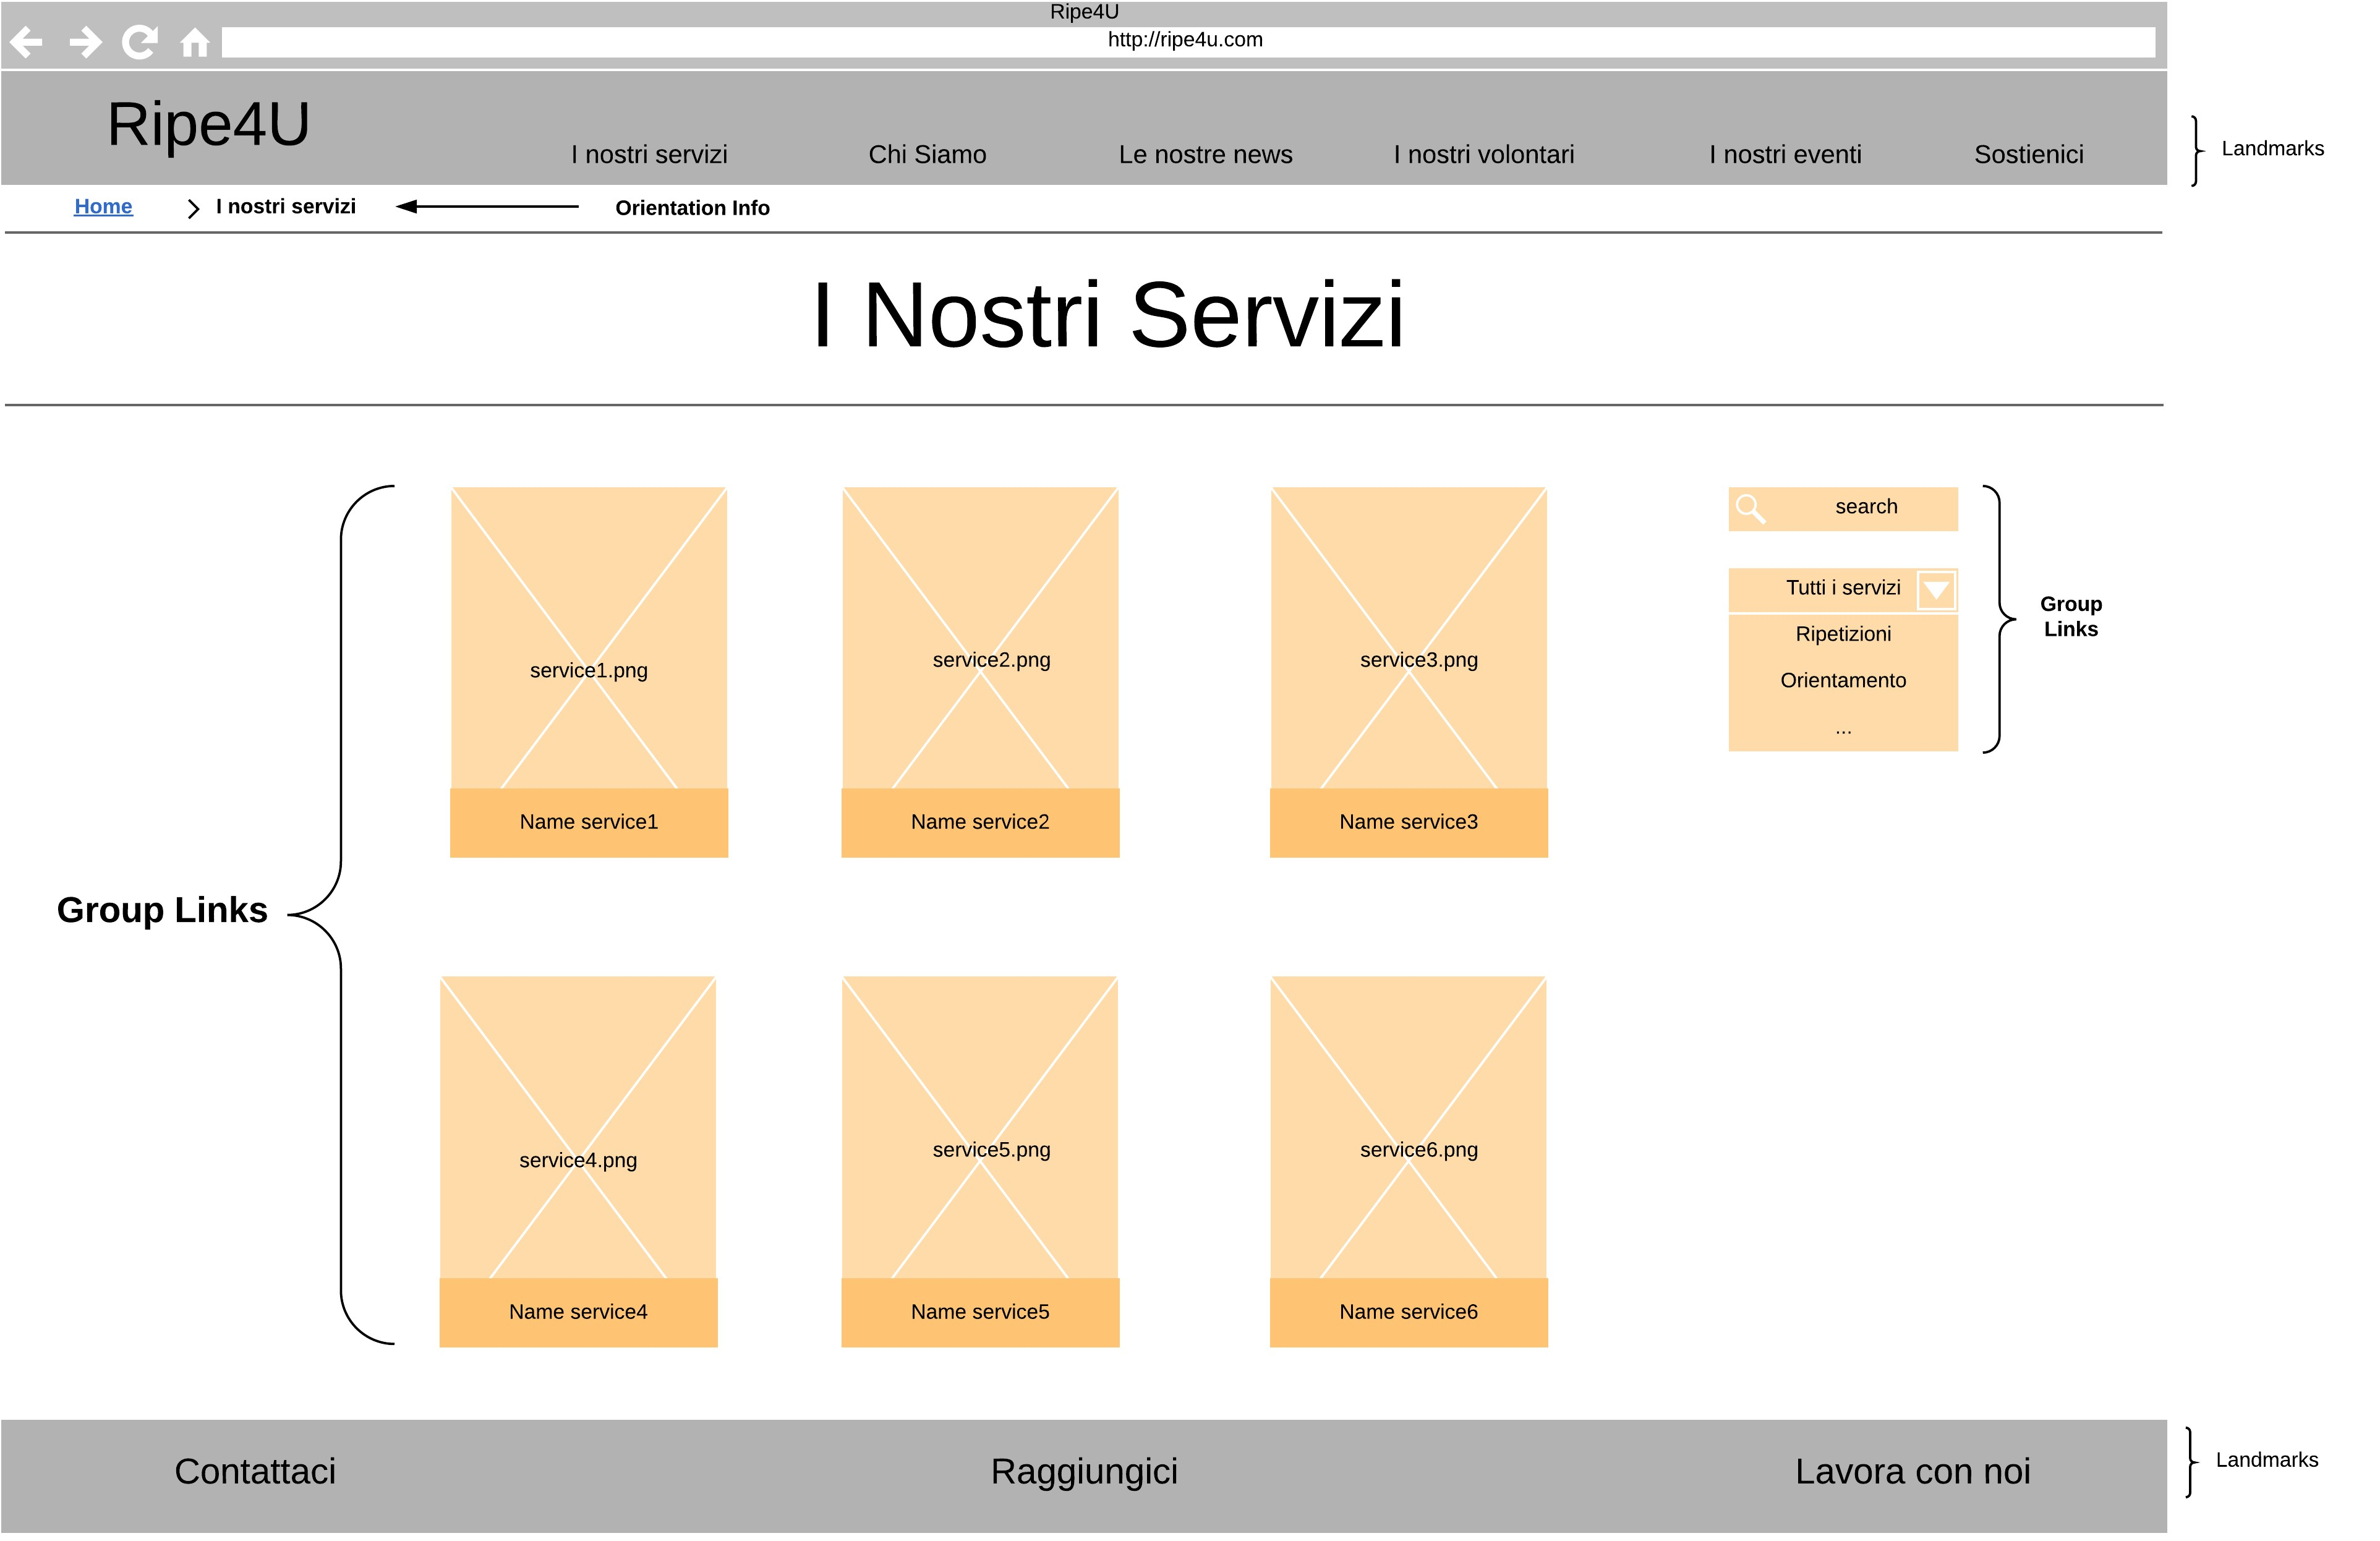
\includegraphics[scale=0.45]{resources/images/iNostriServizi-in-the-small.jpg}
        \end{figure}

        \subsection{I nostri servizi mockup}
    
    \section{Servizio}    
    Questa pagina permette di avere informazioni riguardo al singolo servizio.
    Come primo elemento vediamo una fotografia esplicativa e immediatamente
    sotto due colonne. A destra e a sinistra della fotografia due group link
    permettono di navigare tra le pagine di servizi appartenenti alla stessa
    categoria. Nella colonna di sinistra sotto la fotografia c'è una descrizione
    del servizio e sotto sono presenti delle fotografie dei volontari che si
    occupano dell'erogazione di quel servizio. Cliccando sulle fotografie dei
    volontari e sfruttando appositi transition links è possibile raggiungere le
    loro pagine personali per contattarli. Nella colonna di destra sono presente
    gli eventuali eventi in cui è possibile trovare il servizio. Cliccando sulla
    fotografia dell'eventi e sfruttando gli appositi transition links si
    raggiungono le pagine degli eventi.

        \subsection{Servizio in-the-small}
        \begin{figure}[H]
            \centering
            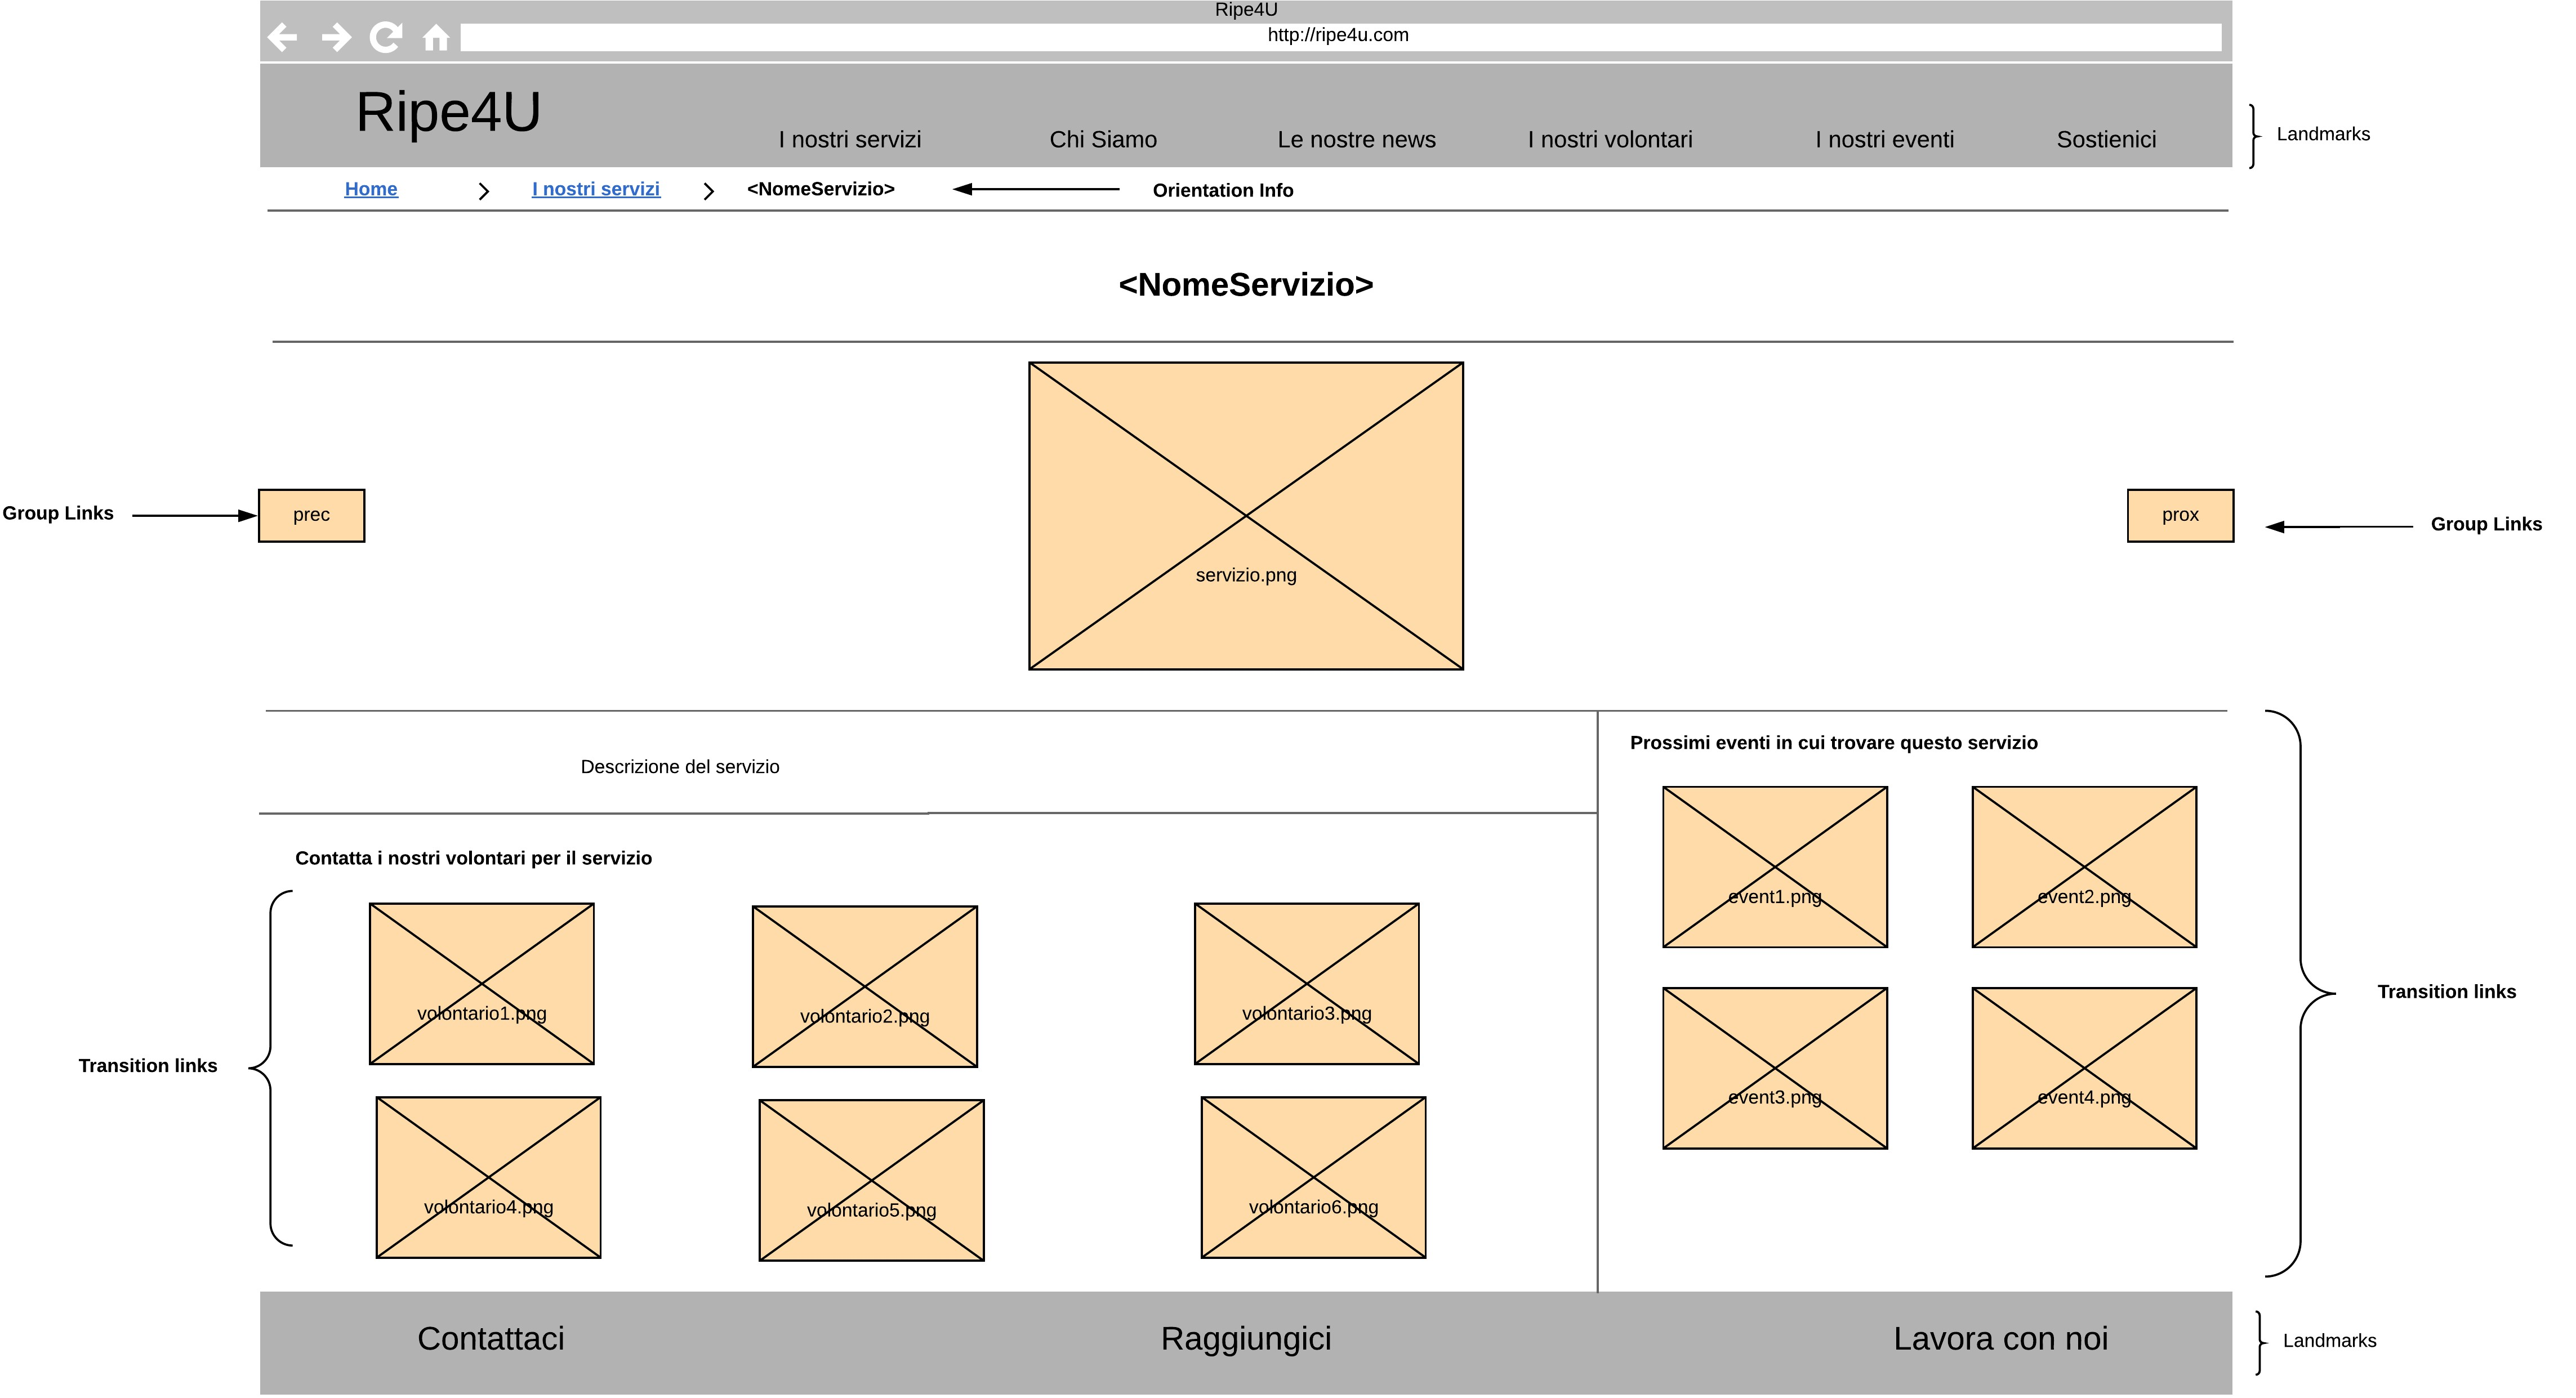
\includegraphics[scale=0.37]{resources/images/servizio-in-the-small.jpg}
        \end{figure}

        \subsection{Servizio mockup}

    \section{I nostri eventi}
    Questa pagina permette di mostrare tutti gli eventi che l'associazione
    organizza. Nella pagina sono presenti delle foto esplicativo con il nome
    dell'evento. Nella parte destra della pagina è presente una barra di ricerca
    che permette di cercare un evento specifico come "vacanza studio in
    montagna". Sotto la barra di ricerca sono presenti dei filtri che permettono
    di mostrare gli eventi in base alla tipologia come "Vacanze studio" oppure
    "Feste insieme". Cliccando sulle fotografie è possibile raggiungere le
    pagine dei singoli eventi sfruttando appositi group link.

        \subsection{I nostri eventi in-the-small}
        \begin{figure}[H]
            \centering
            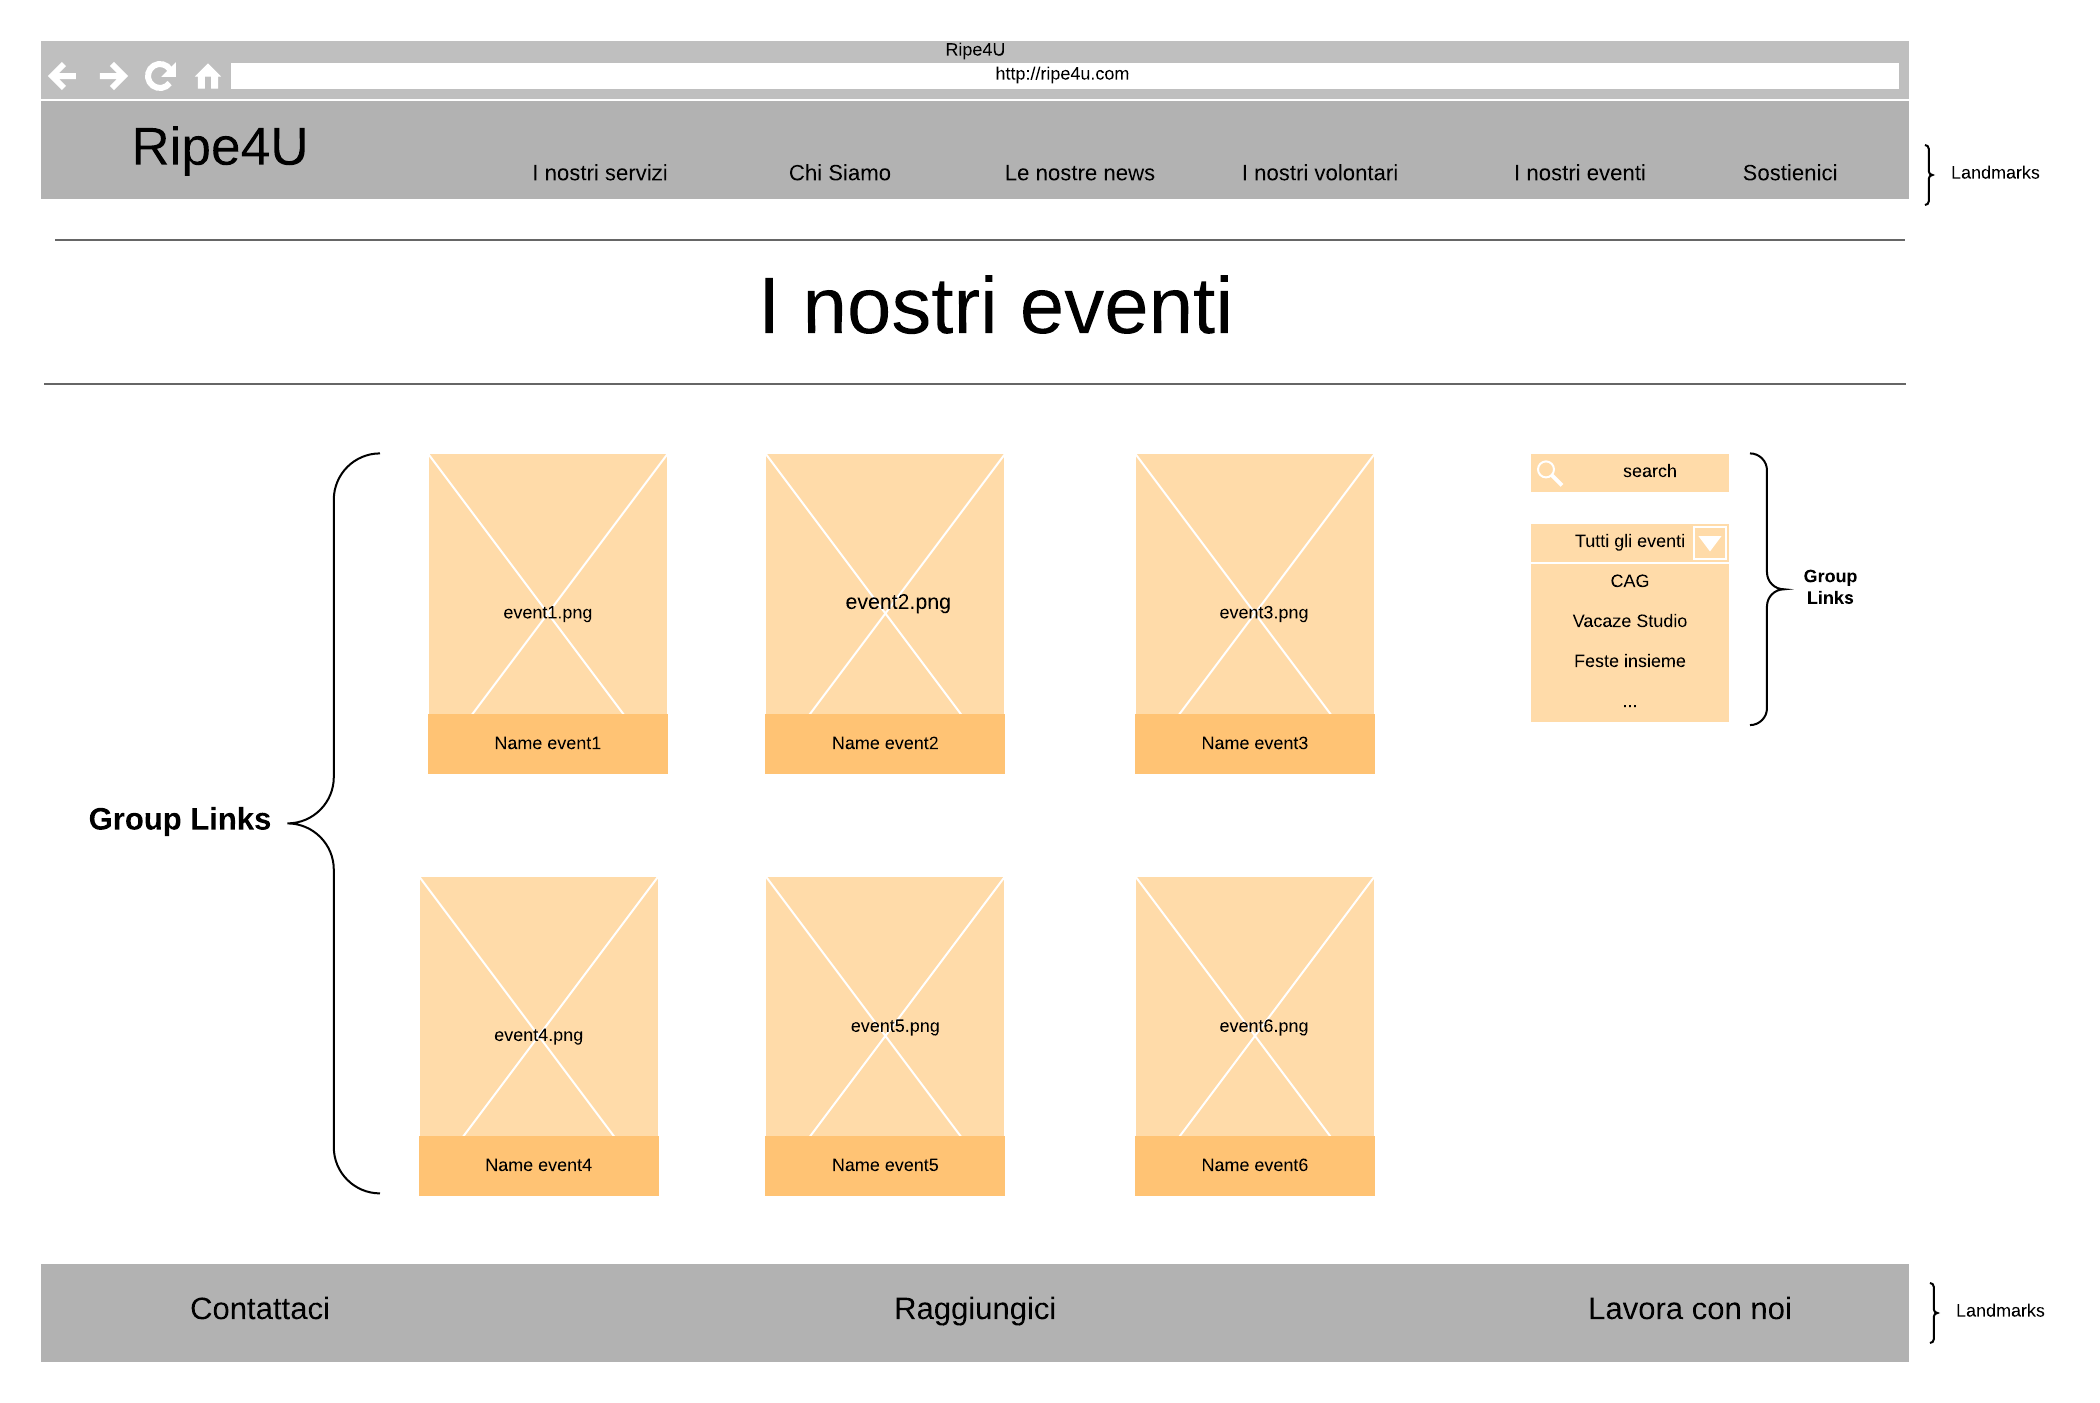
\includegraphics[scale=0.37]{resources/images/iNostriEventi-in-the-small.jpg}
        \end{figure}

        \subsection{I nostri eventi mockup}
    
    \section{Evento}
    Questa pagina permette di avere informazioni riguardo al singolo evento.
    Come primo elemento vediamo una fotografia esplicativa dell'evento con a
    destra e a sinistra due group link che permettono di navigare tra le pagine
    di eventi appartenenti alla stessa categoria. Sotto la fotografia ci sono
    due colonne. Nella colonna di sinistra ci sono una descrizione dell'evento,
    la data e il luogo dell'evento, una fotografia del volontario responsabile
    per l'evento e informazioni riguardo ai posti disponibili con la possibilità
    di inserire la mail personale per prenotare un posto. Cliccando sulla
    fotografia del responsabile e sfruttando l'apposito transition link si
    raggiungere la pagina del volontario incaricato dell'organizzazione
    dell'evento. Nella colonna di sinistra sono presenti gli eventuali servizi
    erogati durante l'evento. Se ad esempio l'evento riguarda delle vacanze
    studio tra i servizi possiamo trovare tutte le diverse ripetizioni che i
    volontari proporrano durante il periodo in vacanza. Cliccando sulla foto del
    singolo servizio e sfruttando l'apposito transition link si raggiunge la
    pagina specifica del servizio.

        \subsection{Evento in-the-small}
        \begin{figure}[H]
            \centering
            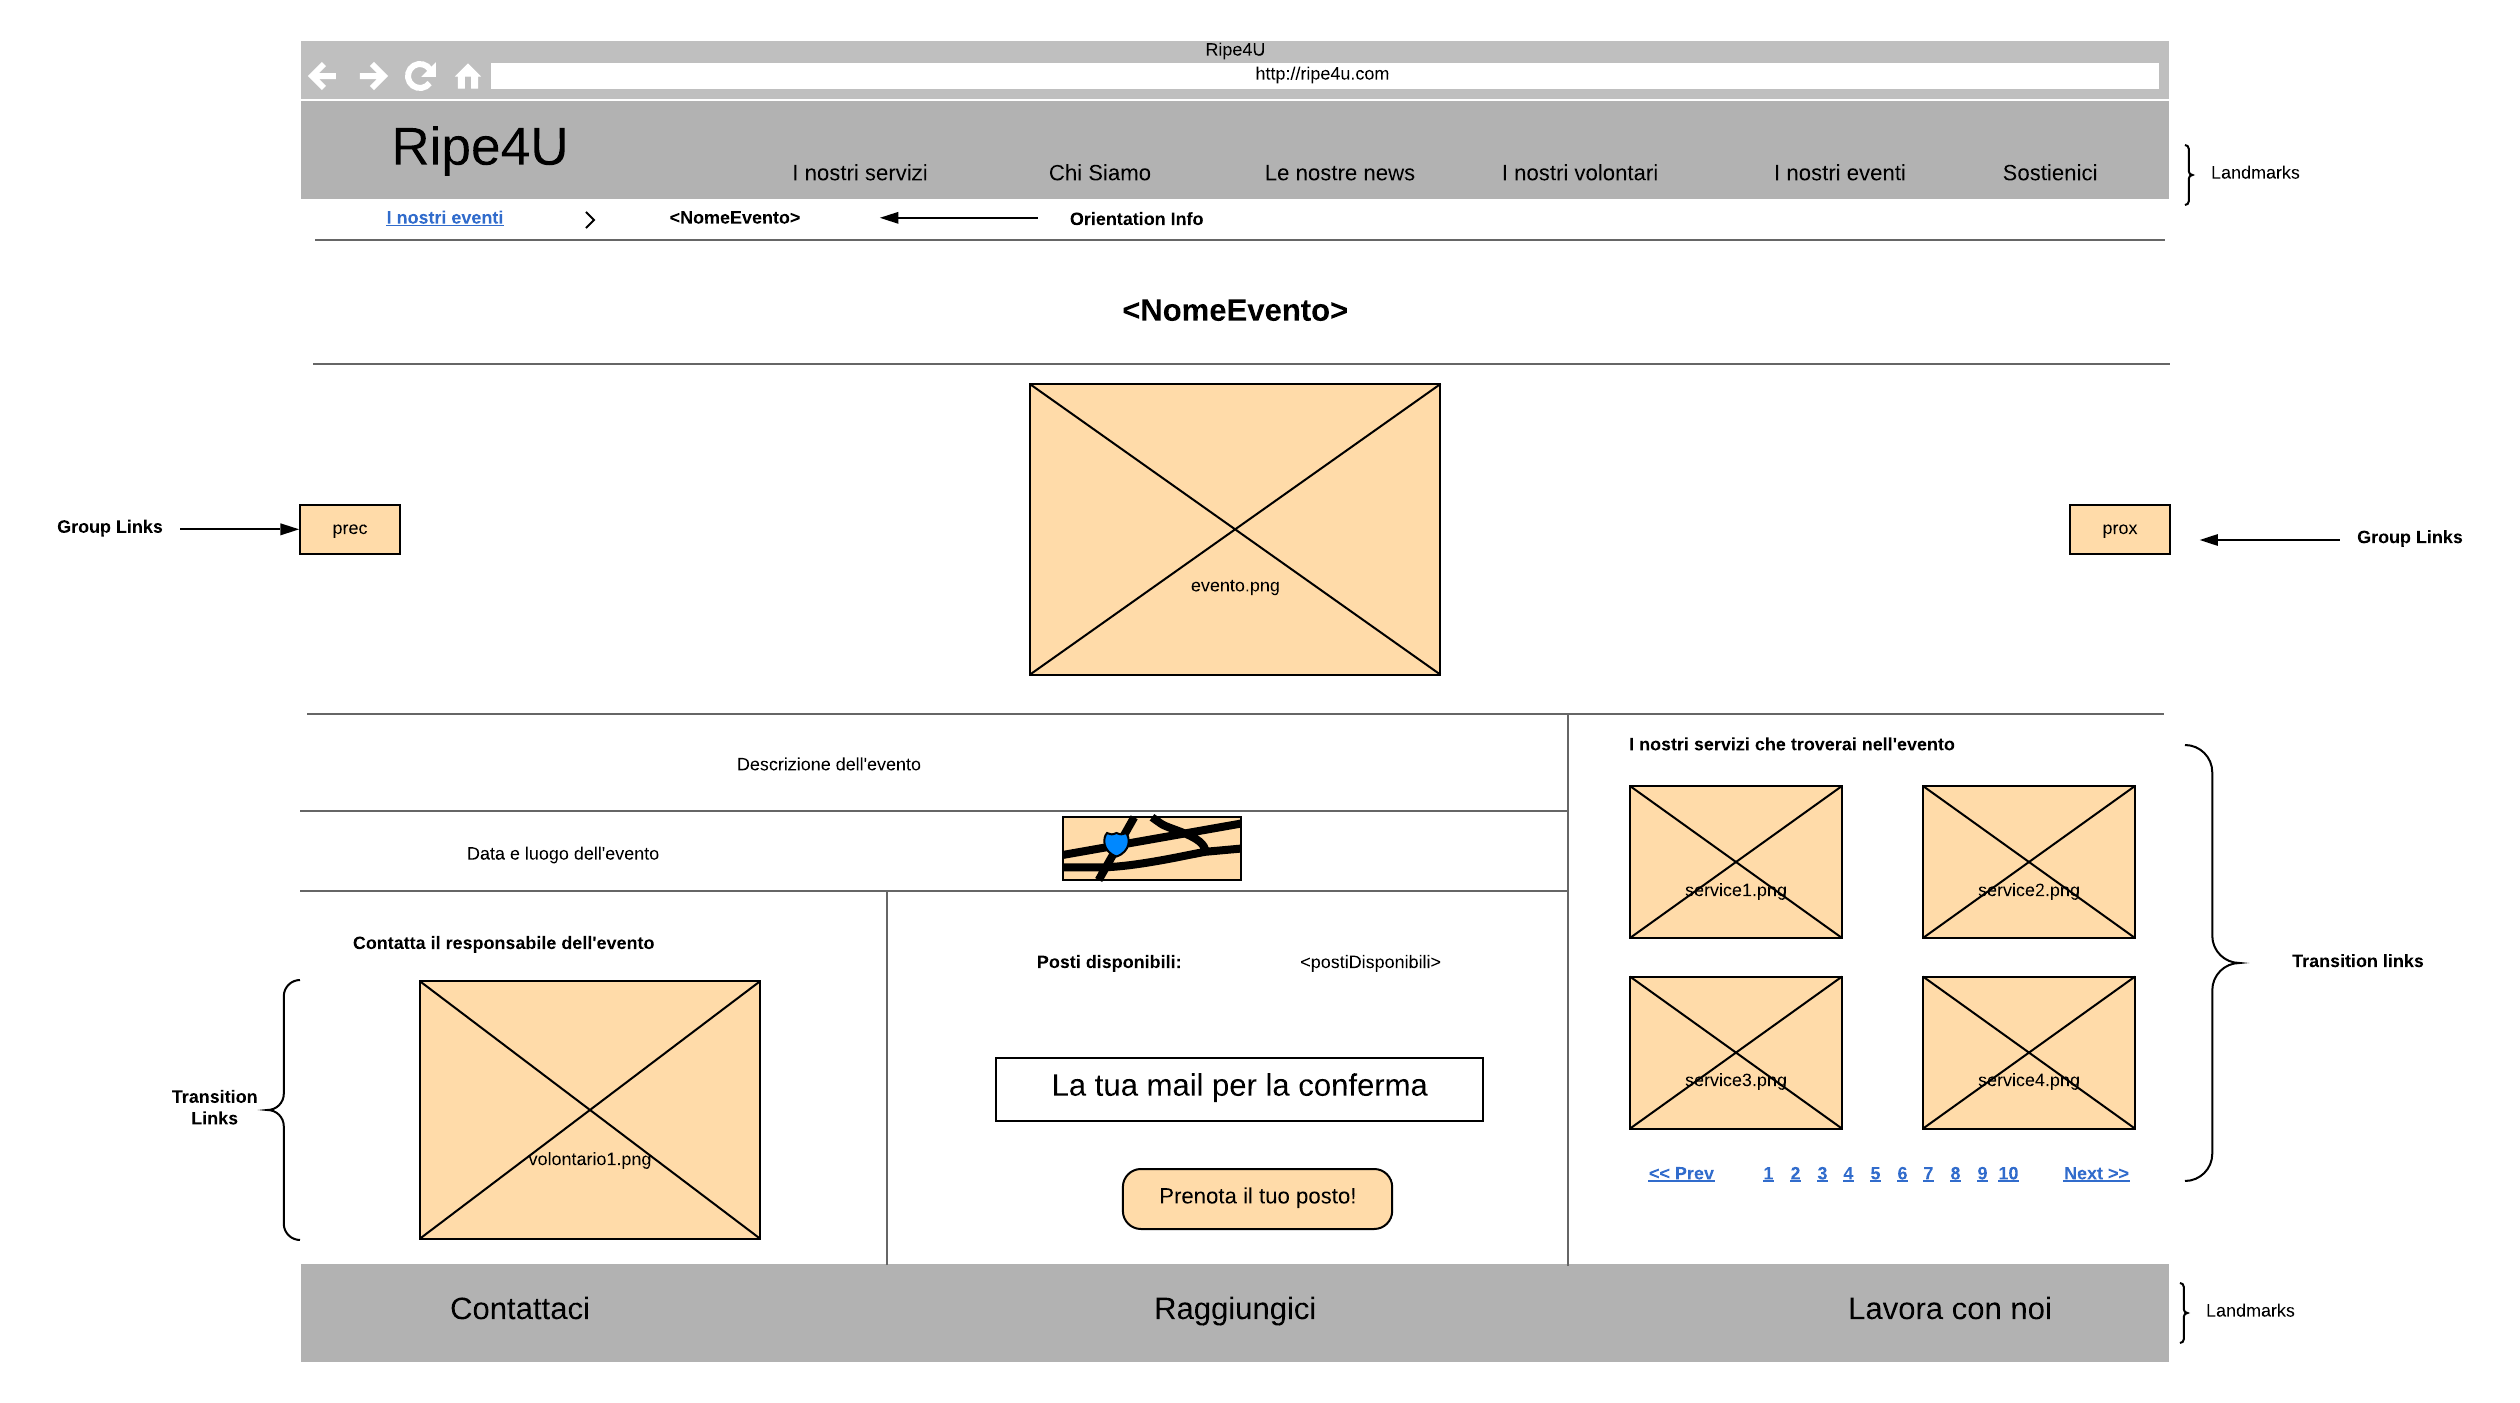
\includegraphics[scale=0.37]{resources/images/evento-in-the-small.jpg}
        \end{figure}

        \subsection{Evento mockup}

    \section{Contattaci}
    In questa pagina abbiamo due tab: una identifica la sezione "I nostri
    contatti" dove sono mostrati tutti i contatti come i numeri di telefono e i
    link social. Nella tab "Scrivici" è presente un form che permette all'utente
    di mandare una mail direttamente all'associazione per richiedere
    informazioni.

        \subsection{Contattaci in-the-small}
        \begin{figure}[H]
            \centering
            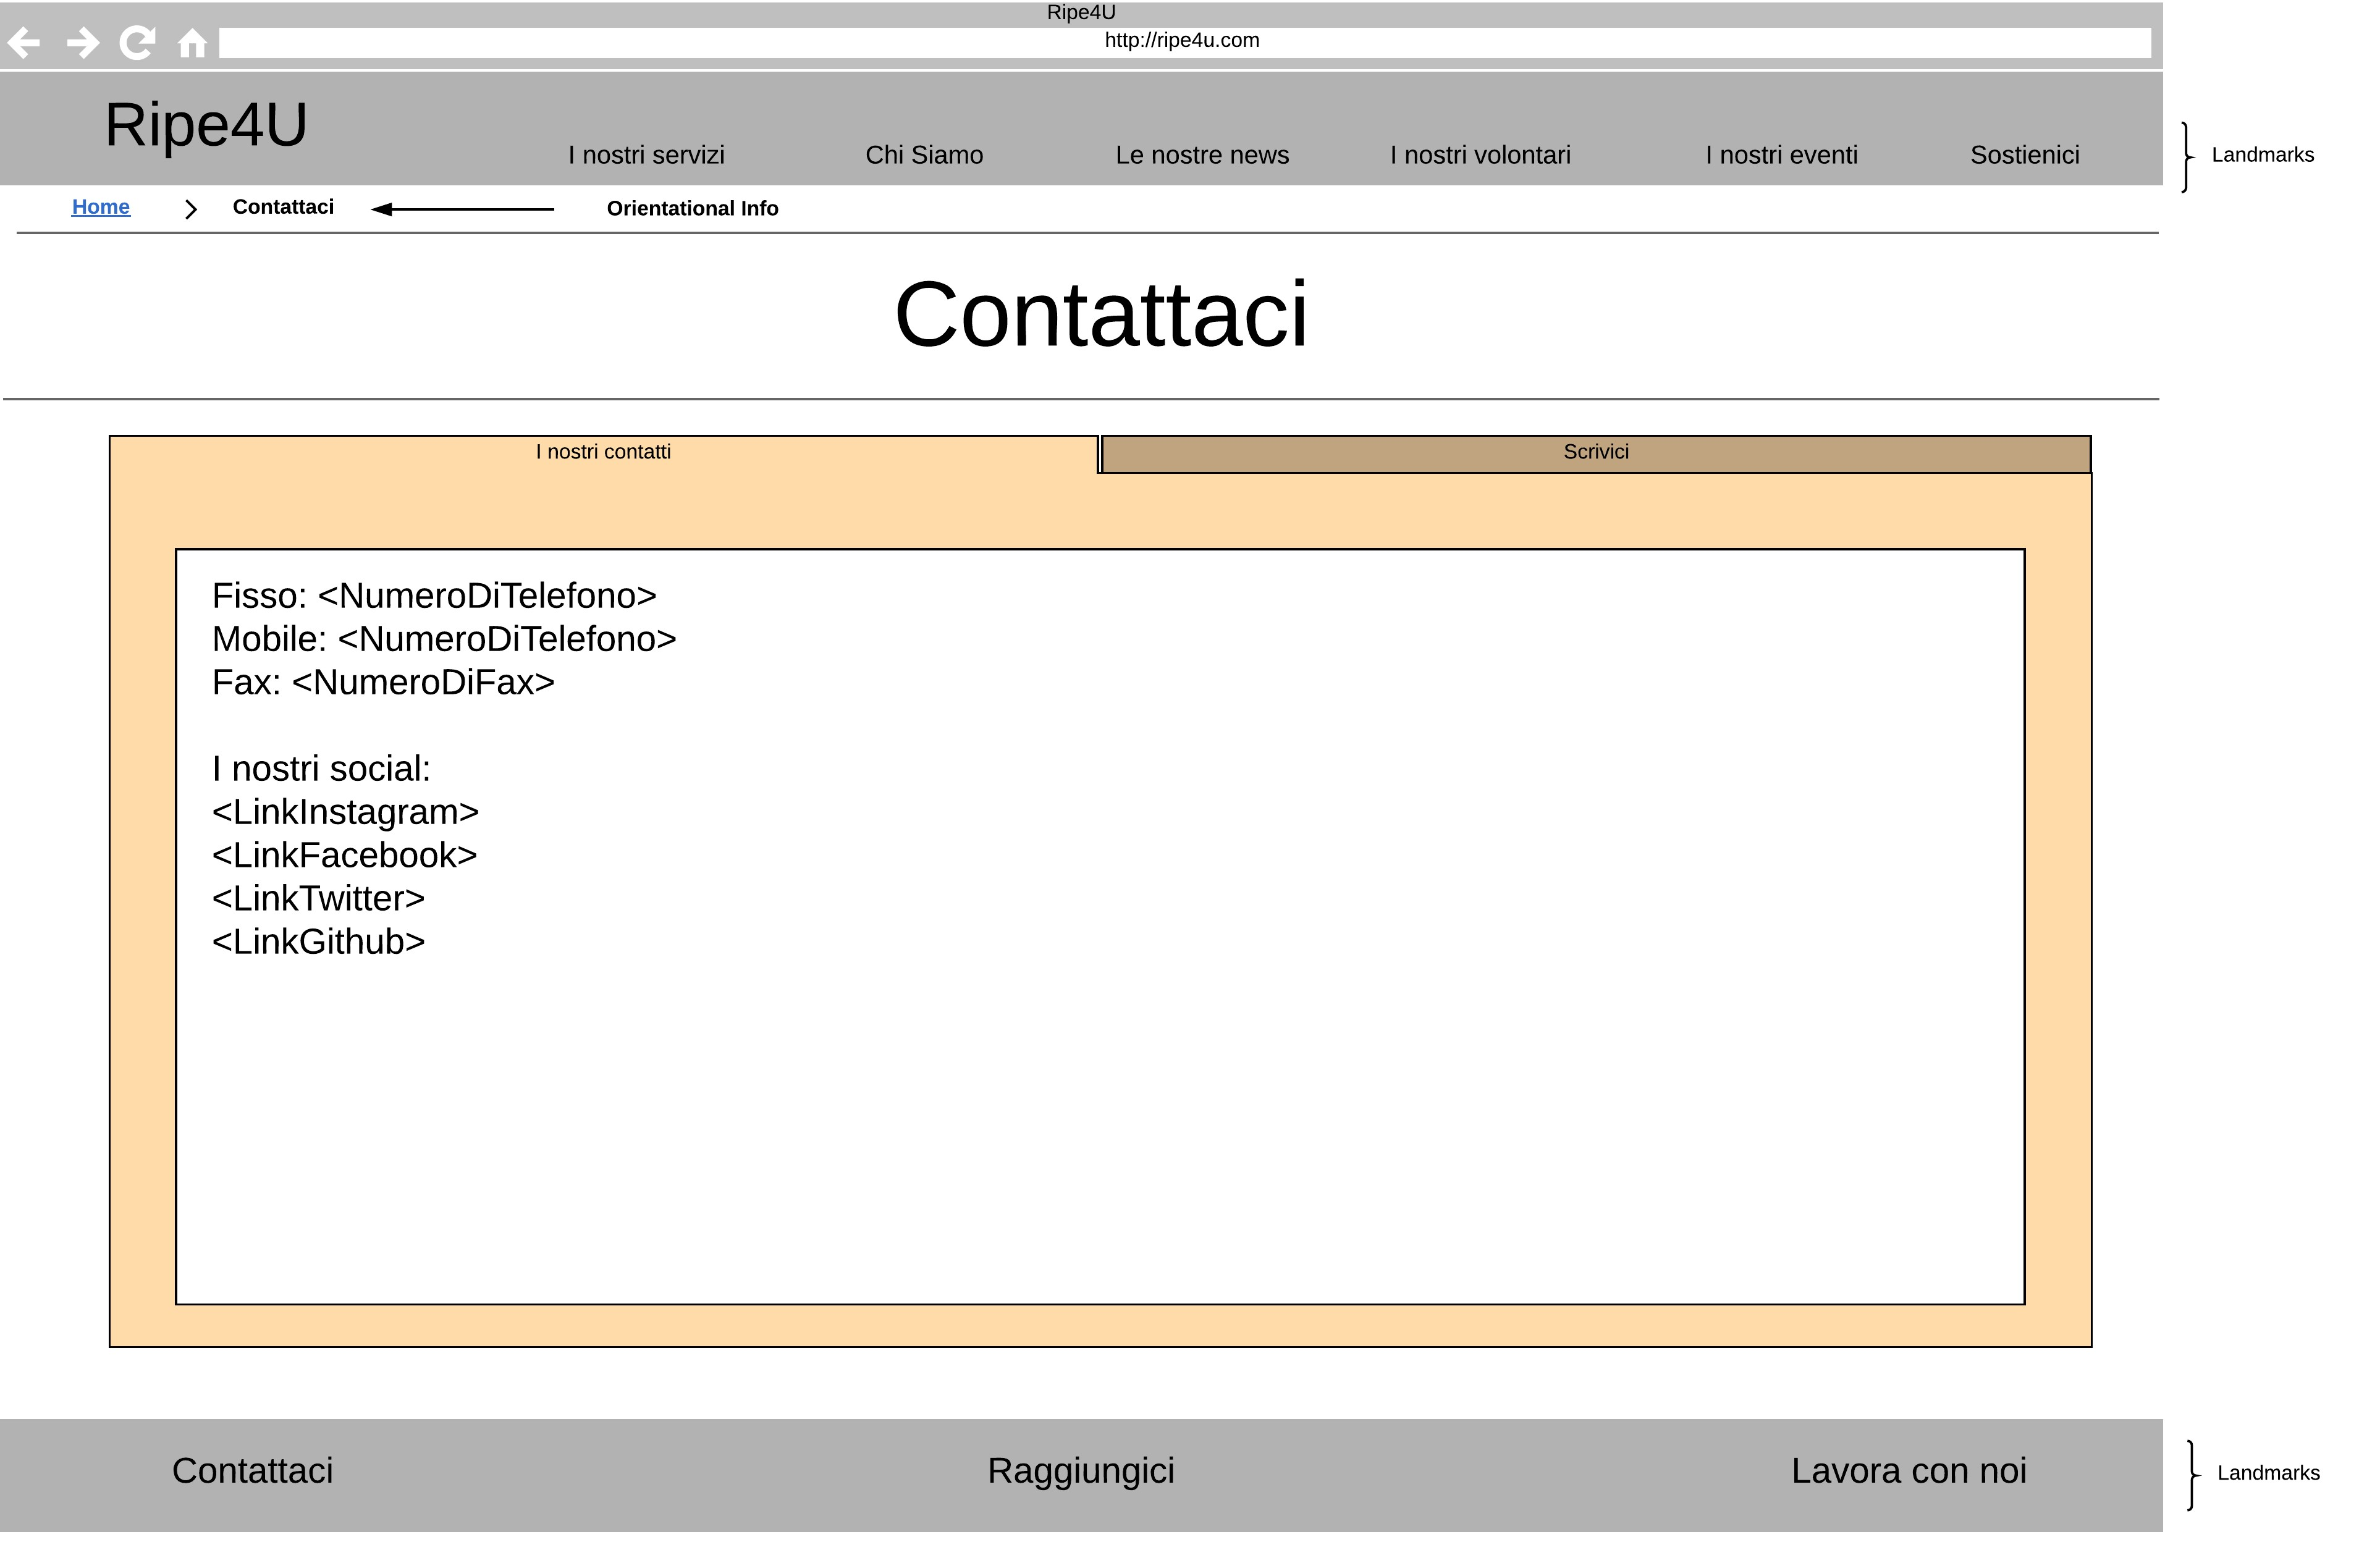
\includegraphics[scale=0.37]{resources/images/contattaci1-in-the-small.jpg}
        \end{figure}
        \begin{figure}[H]
            \centering
            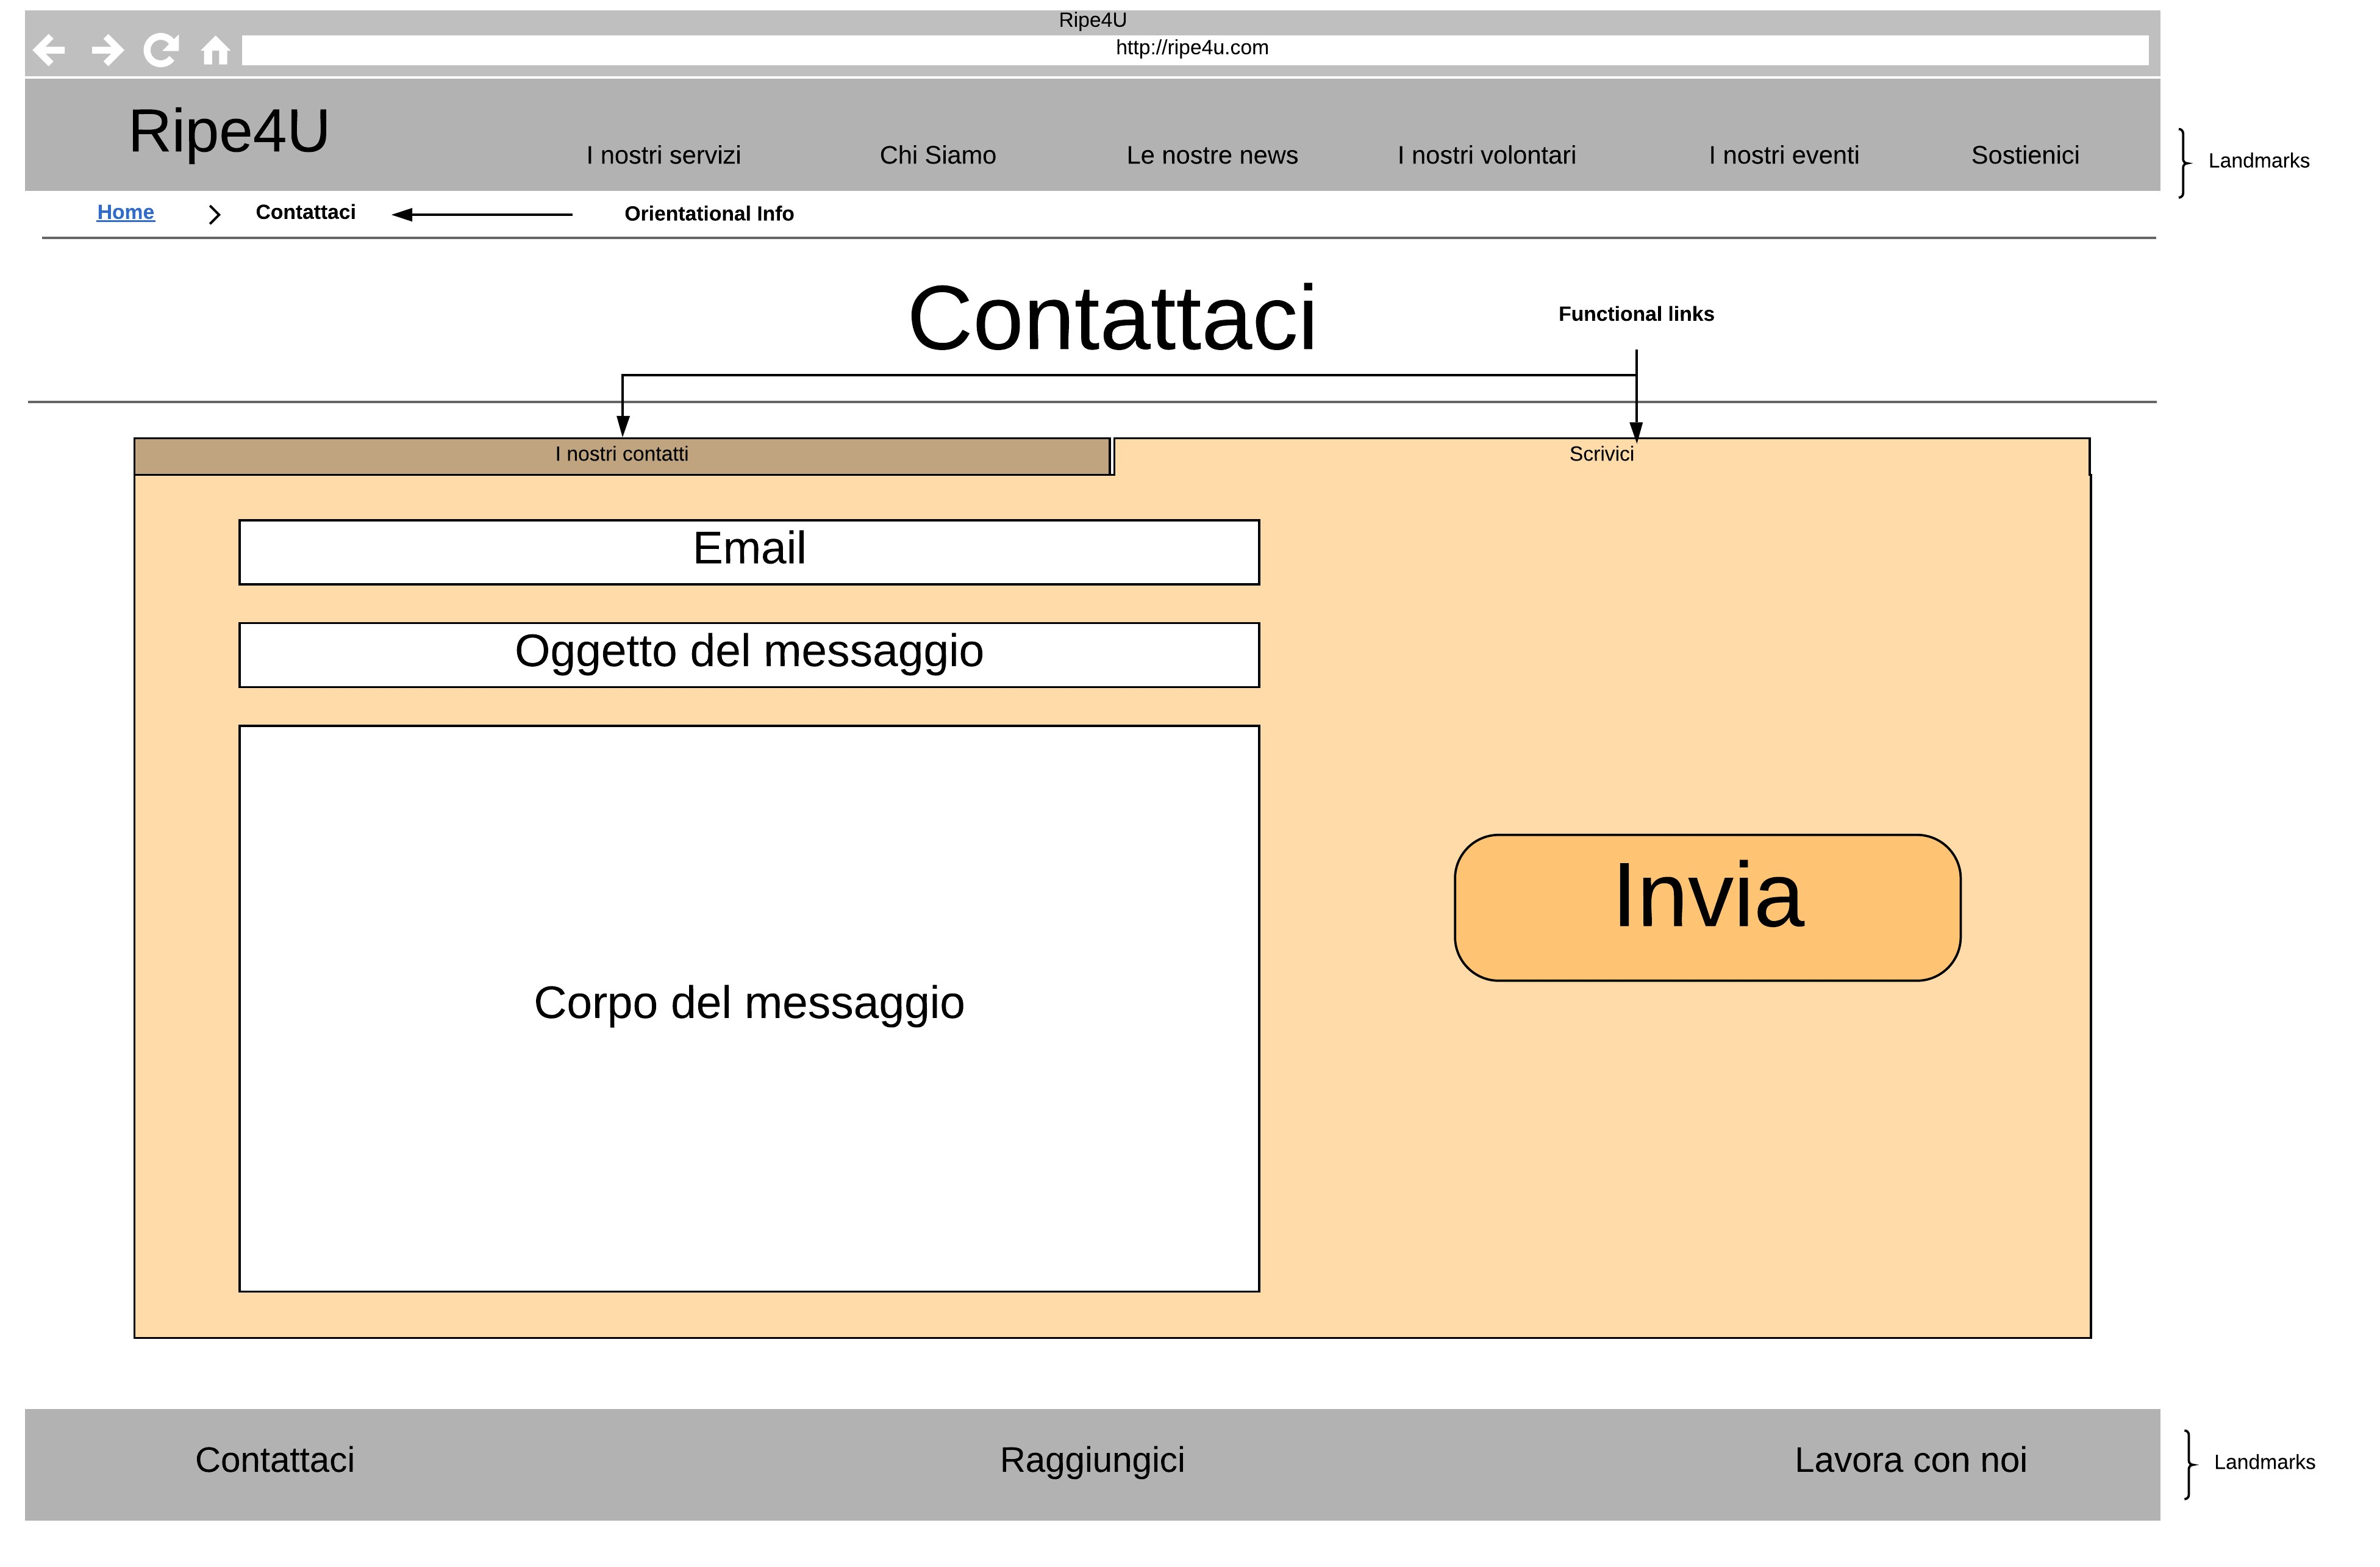
\includegraphics[scale=0.37]{resources/images/contattaci2-in-the-small.jpg}
        \end{figure}

        \subsection{Contattaci mockup}
    
    \section{News}
    In questa pagina sono mostrate le immagini e i nomi delle news più recenti.
    Cliccando sulle immagini e sfruttando appositi group links è possibile
    raggiungere le pagine delle singole news. Nella parte destra della pagina è
    presente una barra di ricerca.

        \subsection{News in-the-small}
        \begin{figure}[H]
            \centering
            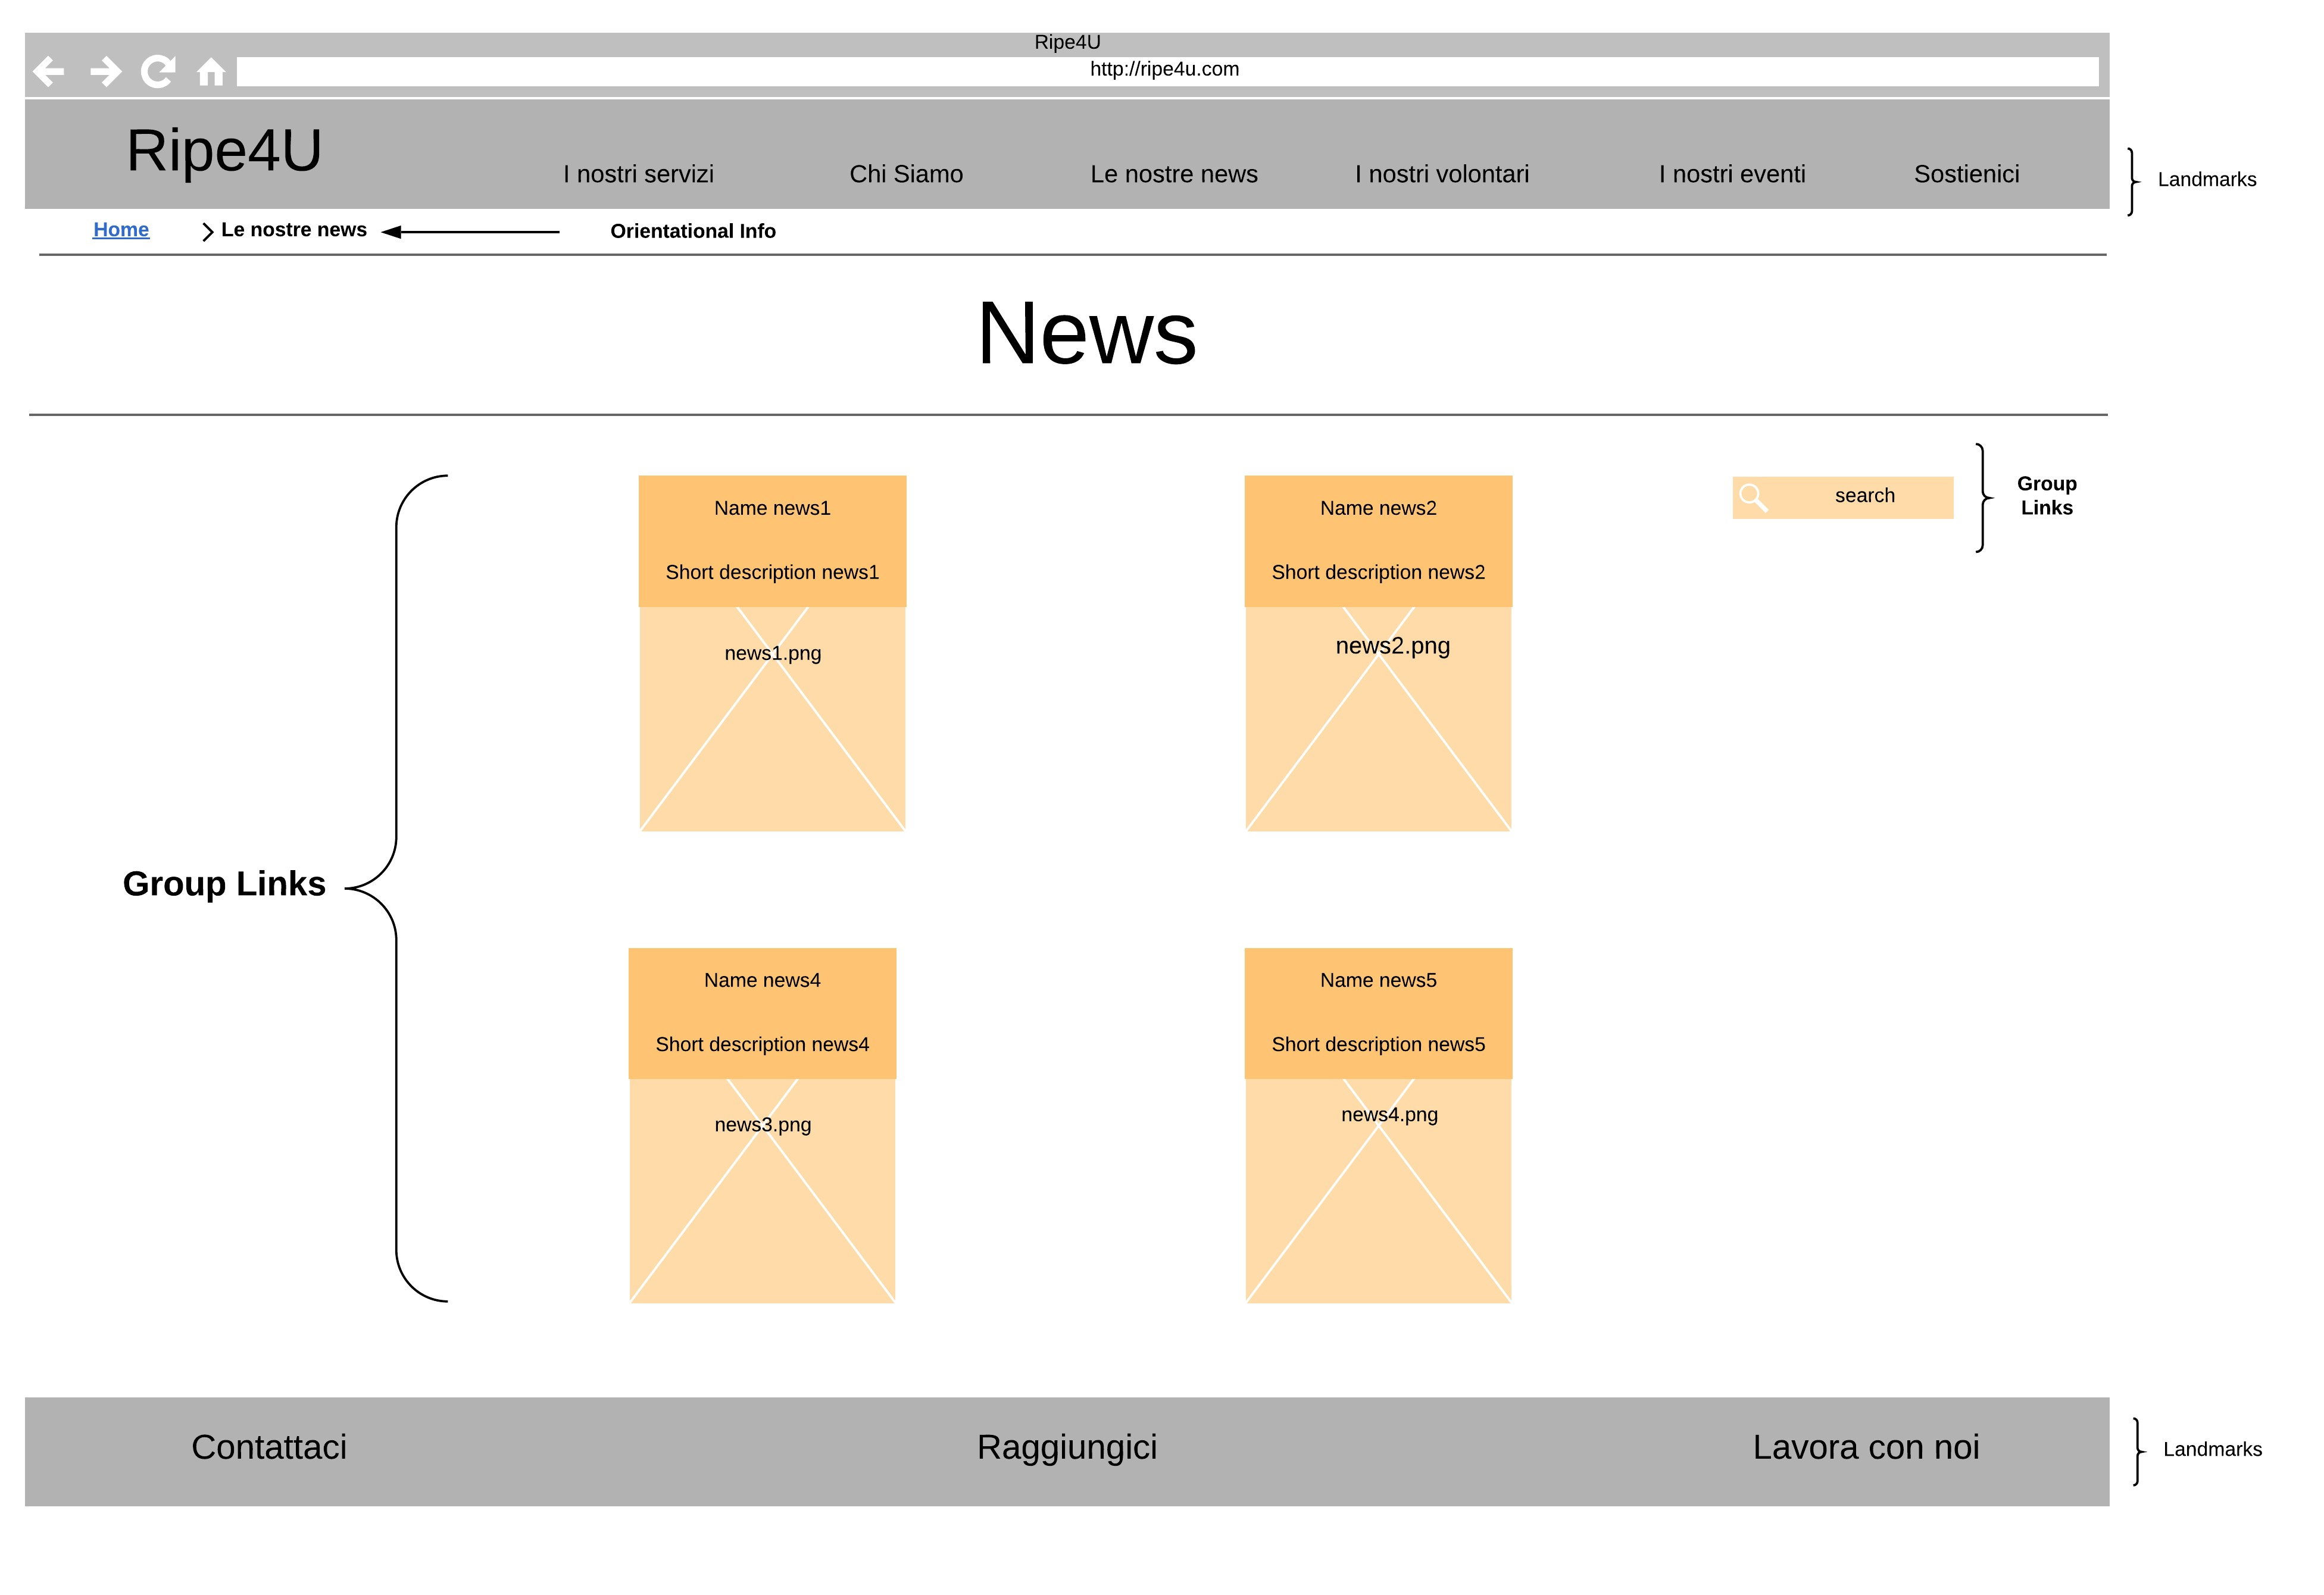
\includegraphics[scale=0.37]{resources/images/news-in-the-small.jpg}
        \end{figure}

        \subsection{News mockup}
    
    \section{Singola news}
    In questa pagina viene riportati la singola news nella sua interezza. Come
    primo elemento è presente un'immagine che identifica la news e alla sua
    destra e sinistra sono presenti dei group link che ci permettono di navigare
    tra le news ordinate cronologicamente. Sotto la fotografia c'è la
    descrizione testuale della news.

        \subsection{Singola news in-the-small}
        \subsection{News in-the-small}
        \begin{figure}[H]
            \centering
            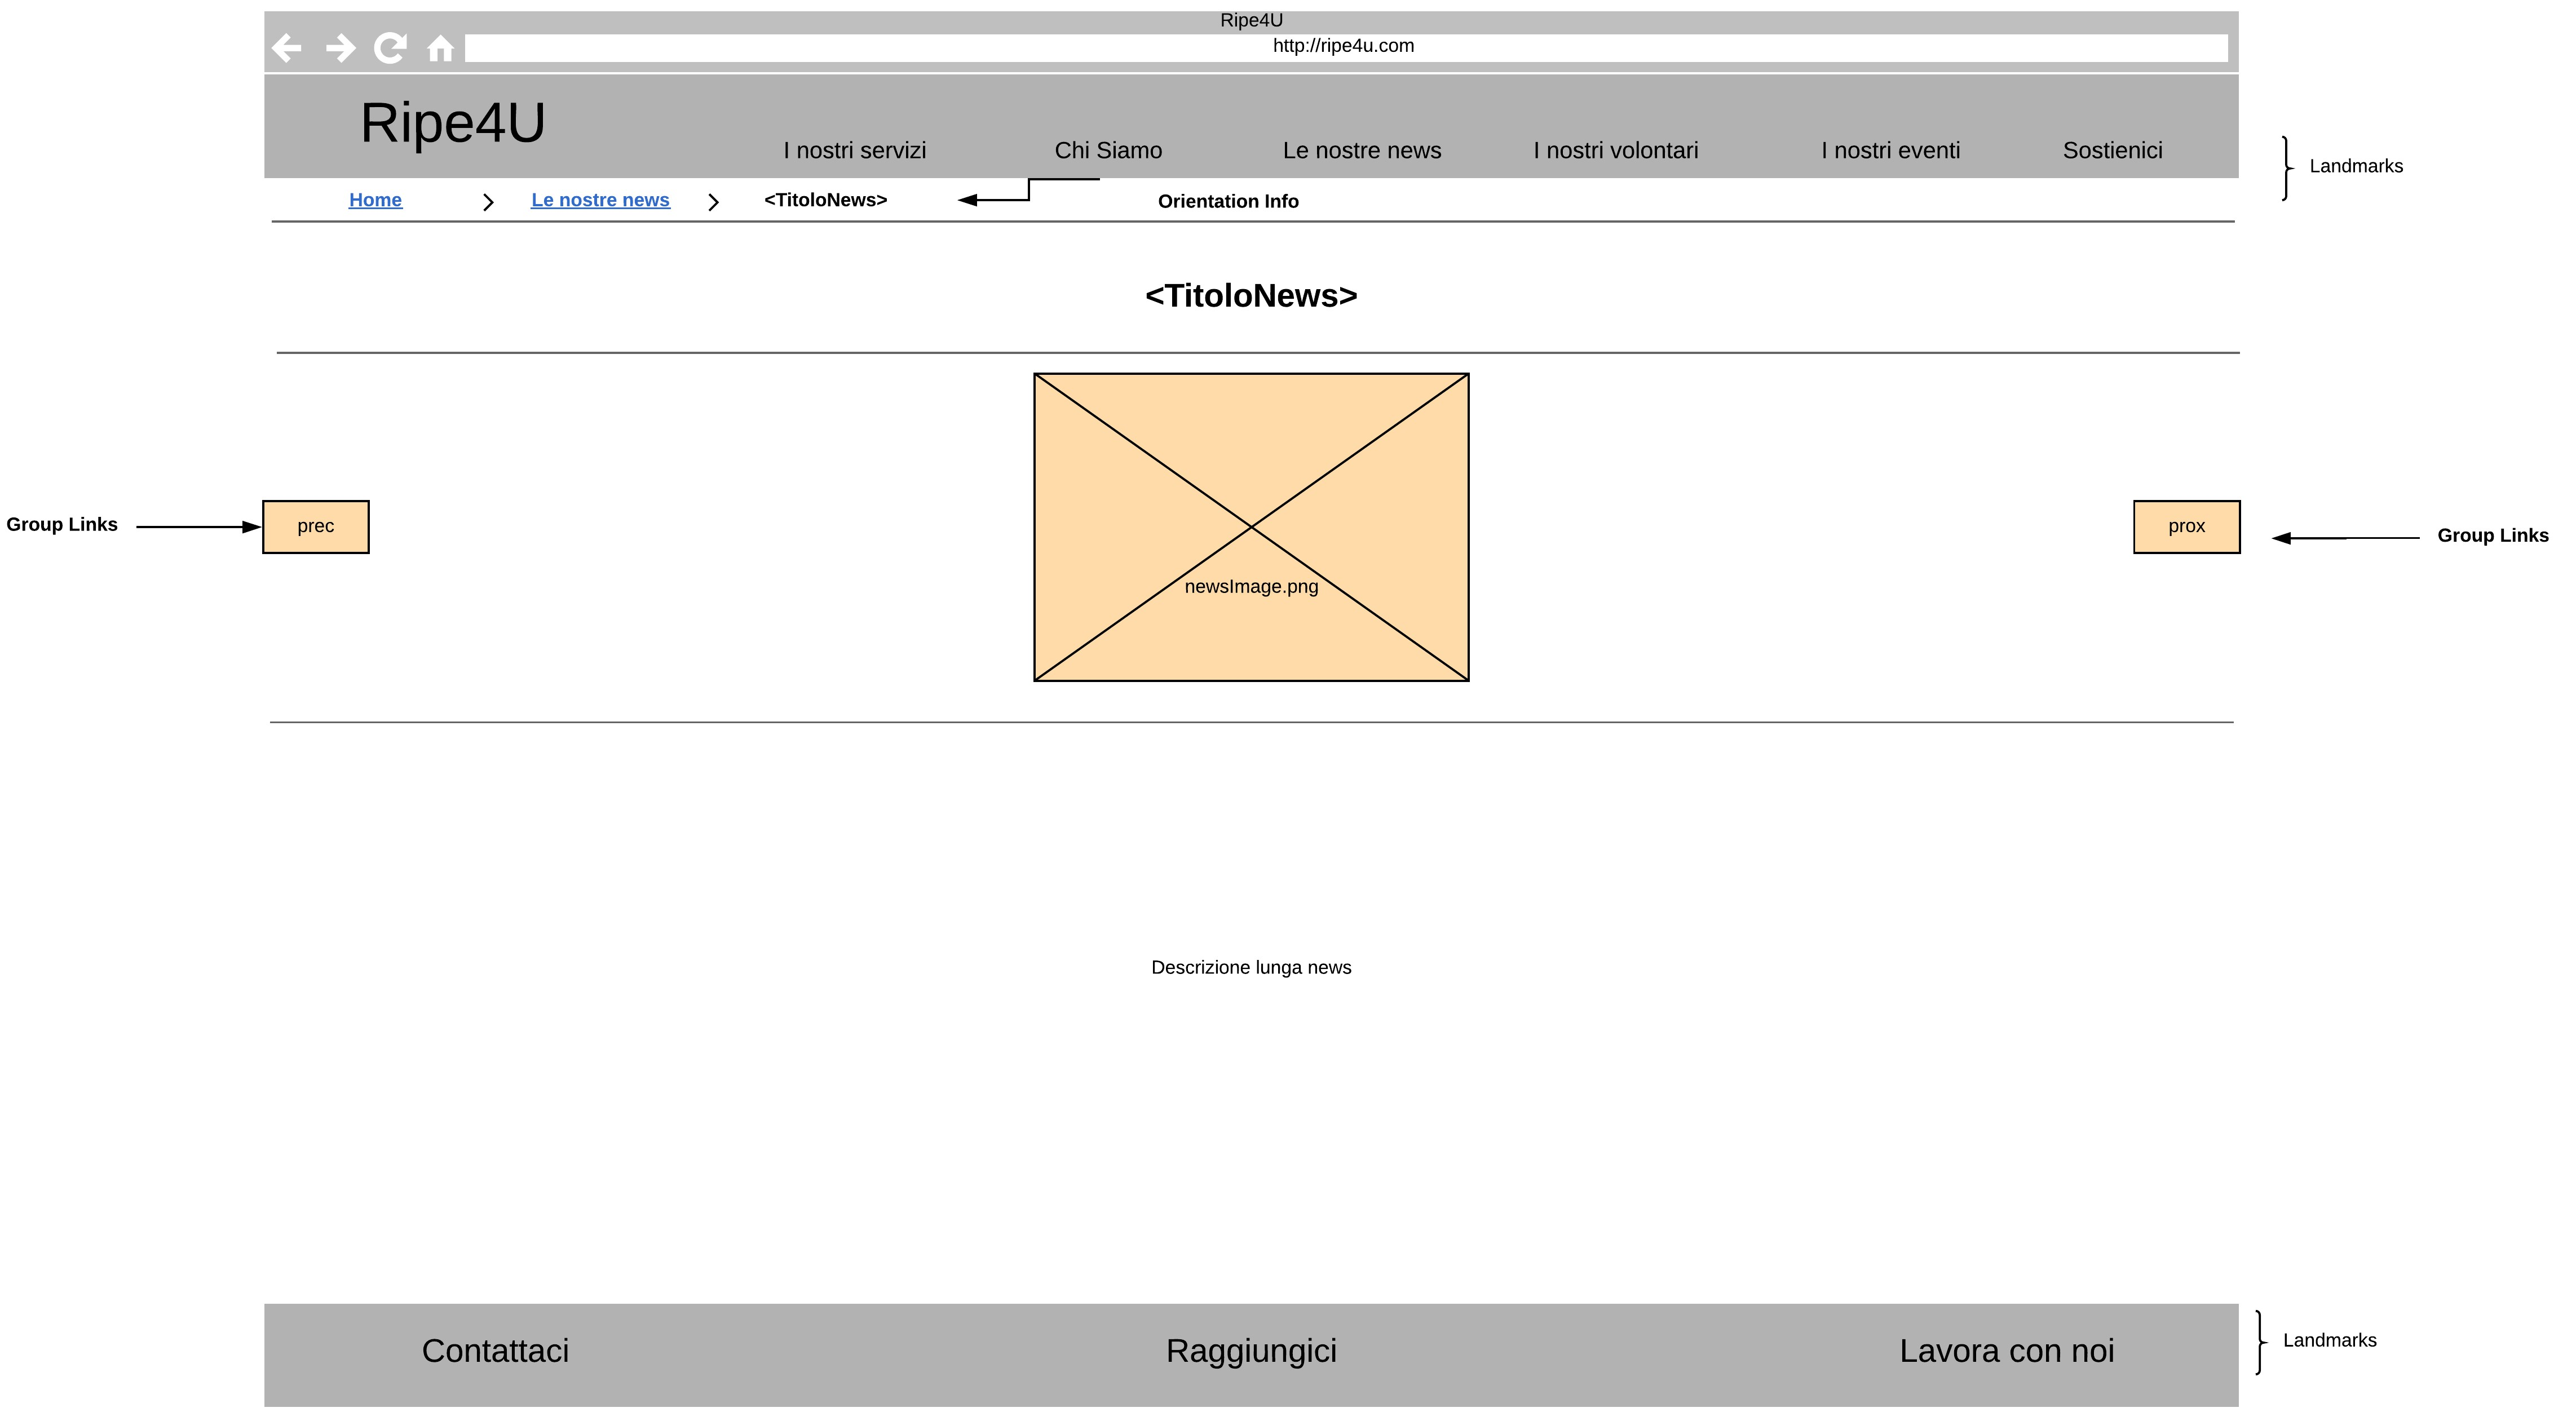
\includegraphics[scale=0.37]{resources/images/singolaNews-in-the-small.jpg}
        \end{figure}

        \subsection{Singola news mockup}

    \section{Homepage}
    L'homepage del sito presenta uno slideshow dove vengono mostrate alcune foto
    esemplificative delle attività svolte dall'associazione. Immediatamente
    sotto lo slideshow c'è una descrizione testuale di tutto quello che fa
    l'associazione. Come ultimo elemento nella pagina sono riportate le quattro
    notizie più recenti. Cliccando sui transition link della fotografie delle
    notizie si raggiunge la pagina dedicata alle singole notizie.
        
        \subsection{Homepage in-the-small}
        \begin{figure}[H]
            \centering
            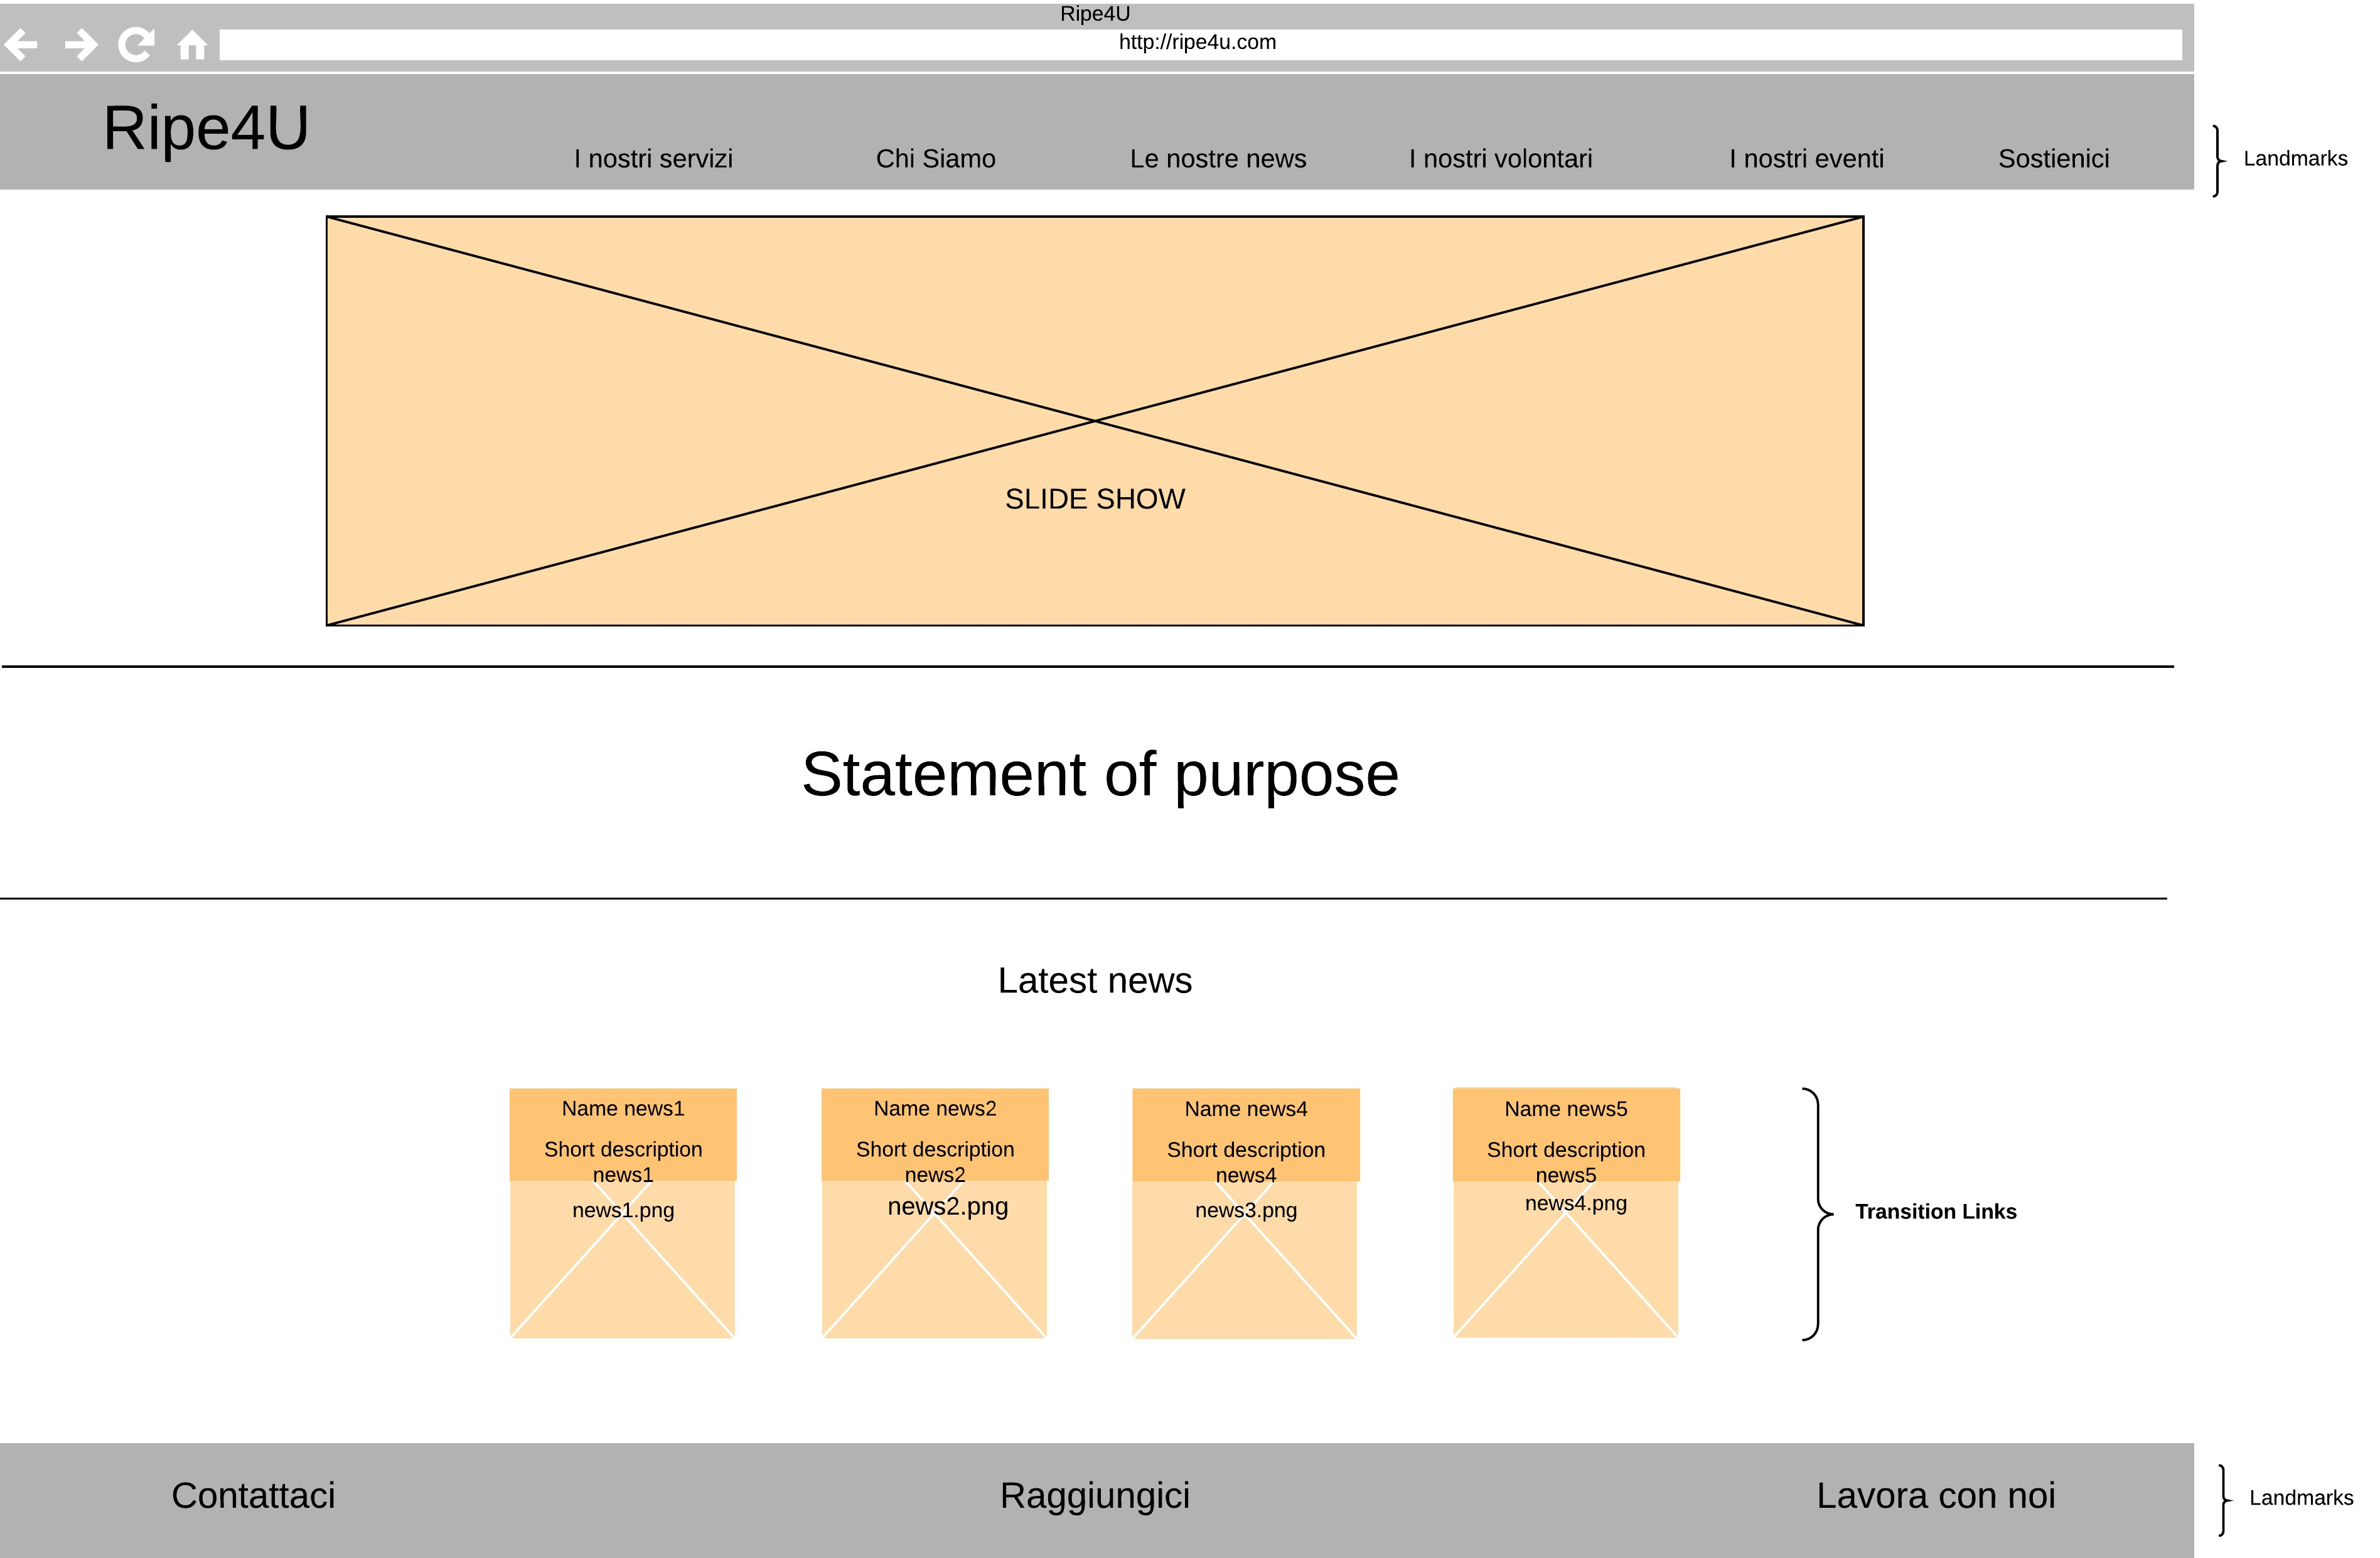
\includegraphics[scale=0.37]{resources/images/homepage-in-the-small.jpg}
        \end{figure}
        \subsection{Homepage mockup}


    